\documentclass[12pt]{article}
\usepackage[english]{babel}
\usepackage[utf8]{inputenc}

\usepackage{hyperref}
\usepackage{booktabs}
\usepackage{tikz}
\usetikzlibrary{positioning}

\newcommand{\tth}[1]{\footnote{\textcolor{blue}{#1}}}
\newcommand{\tbh}[1]{\textsc{\textbf{#1}}}

\title{Technical Report:\\
       Exploring Automatic Model-Checking of the Ethereum specification}
\author{
    Igor Konnov\thanks{This work was supported by Ethereum Foundation
    under grant NNN.}\\ \small Independent Researcher \& TU Wien \\
    \and
    Jure Kukovec\footnotemark[1] \\ \small Independent Researcher \\
    \and
    Thomas Pani\footnotemark[1] \\ \small Independent Researcher\\
    \and
    Roberto Saltini \\ \small Consensys \\
    \and
    Thanh Hai Tran \\ \small Consensys
}
\date{\today}

\usepackage{mathpartir}
\usepackage{amsthm}
\usepackage{amsmath}
\usepackage{amssymb}
\usepackage{mathtools}
\usepackage{listings}
\usepackage{tlalatex}

\newcommand{\SpecOne}{\texttt{Spec~1}}
\newcommand{\SpecTwo}{\texttt{Spec~2}}
\newcommand{\SpecThree}{\texttt{Spec~3}}
\newcommand{\SpecFour}{\texttt{Spec~4}}
\lstset{%
  basicstyle=\sffamily\scriptsize,   % Use a variable-width font
  columns=fullflexible,   % Adjust spacing to match the variable-width font
  frame=single,           % Only around the code
}

\lstdefinelanguage{tla}{%
  morekeywords={MODULE,EXTENDS,CONSTANTS,CONSTANT,ASSUME,VARIABLES,VARIABLE,
          EXCEPT,UNCHANGED,TRUE,FALSE,IF,THEN,ELSE,LET,IN,SUBSET,DOMAIN,RECURSIVE},
          comment=[l]{\\*},
  morecomment=[s]{(*}{*)},
  mathescape=true,escapechar={@},
  commentstyle=\itshape\rmfamily,%\small,
  keywordstyle=\sffamily\bfseries
}
\lstdefinelanguage{alloy}{%
  morekeywords={pred,sig,fact,set,one,extends,all,or,and,run,for,but},
          comment=[l]{---},
  mathescape=true,escapechar={@},
  basicstyle=\sffamily,%\small,
  commentstyle=\itshape\rmfamily,%\small,
  keywordstyle=\sffamily\bfseries
}

\lstdefinelanguage{smt}{%
    keywords={%
        assert, check-sat, get-model, set, define-fun, define-fun-rec,
        not, or, and, ite, let, forall, exists, true, false
    },
    alsoletter=-,
    morekeywords={%
        declare-const, define-sort, check-sat, set-option,
        get-assertions, get-info, get-value, set-logic,
        declare-datatypes, declare-datatype, declare-fun
    },
    sensitive=true,
    comment=[l]{;}, % Single line comments
    morecomment=[s]{(*}{*)}, % Multi-line comments
    string=[b]" % Strings
}

\newtheorem{theorem}{Theorem}[section]
\newtheorem{lemma}[theorem]{Lemma}
\newtheorem{corollary}[theorem]{Corollary}

\newcommand{\iteDef}[4]{
  #1 \coloneqq \left\{
\begin{array}{ll}
      #2 &; #3 \\
      #4 &; \text{otherwise}\\
\end{array} 
\right. 
}

\newcommand{\tlap}{$\textsc{TLA}^{+}$}
% \newcommand{\defeq}{\;\mathrel{\smash   %% keep this symbol from being too tall
%     {{\stackrel{\scriptscriptstyle\Delta}{=}}}}\;}

\newcommand{\nat}{\mathbb N_0}

\newcommand{\op}{\mathrm{R}}
\newcommand{\nrop}{\mathrm{I}}
\newcommand{\mop}{\mathrm{R}_m}
\newcommand{\mapg}{\mathrm{G}_m}
\newcommand{\bb}{\mathrm{next}}
\newcommand{\Chain}{\mathrm{Stack}}

\newcommand{\tup}[1]{\left<\left<#1\right>\right>}
\newcommand{\htau}{\hat{\tau}}

\newcommand{\List}{\mathrm{List}}
\newcommand{\Seq}{\mathrm{Seq}}
\newcommand{\Set}{\mathrm{Set}}
\newcommand{\PVec}{\mathrm{PVec}}
\newcommand{\PSet}{\mathrm{PSet}}
\newcommand{\PMap}{\mathrm{PMap}}
\newcommand{\Concat}{\mathrm{Concat}}
\newcommand{\Callable}{\mathrm{Callable}}
\newcommand{\Le}{\mathrm{Le}}
\newcommand{\bool}{\mathrm{bool}}
\newcommand{\Bool}{\mathrm{Bool}}
\newcommand{\pyint}{\mathrm{int}}
\newcommand{\Int}{\mathrm{Int}}
\newcommand{\ApaFoldSet}{\mathrm{ApaFoldSet}}
\newcommand{\ApaFoldSeqLeft}{\mathrm{ApaFoldSeqLeft}}
\newcommand{\MkSeq}{\mathrm{MkSeq}}
\newcommand{\SetAsFun}{\mathrm{SetAsFun}}
\newcommand{\Push}{\mathrm{Push}}
\newcommand{\At}{\mathrm{At}}
\newcommand{\Indices}{\mathrm{Indices}}
% \newcommand{\UNION}{\mathrm{UNION}}
% \newcommand{\CHOOSE}{\mathrm{CHOOSE}}
% \newcommand{\TRUE}{\mathrm{TRUE}}
% \newcommand{\FALSE}{\mathrm{FALSE}}
% \newcommand{\IF}{\mathrm{IF}}
% \newcommand{\THEN}{\mathrm{THEN}}
% \newcommand{\ELSE}{\mathrm{ELSE}}
% \newcommand{\LET}{\mathrm{LET}}
% \newcommand{\IN}{\mathrm{IN}}
% \newcommand{\DOMAIN}{\mathrm{DOMAIN}}
% \newcommand{\EXCEPT}{\mathrm{EXCEPT}}
% \newcommand{\RECURSIVE}{\mathrm{RECURSIVE}}



% recall a theorem mentioned before with the same label
\newcommand{\recallthm}[2]{%
  {\medskip\noindent\bfseries Theorem~\ref{#1}.~}{\itshape #2}
}
% recall a proposition mentioned before with the same label
\newcommand{\recallproposition}[2]{%
  {\medskip\noindent\bfseries Proposition~\ref{#1}.~}{\itshape #2}
}
% recall a lemma mentioned before with the same label
\newcommand{\recalllemma}[2]{%
  {\medskip\noindent\bfseries Lemma~\ref{#1}.~}{\itshape #2}
}
% recall a corollary mentioned before with the same label
\newcommand{\recallcorollary}[2]{%
  {\medskip\noindent\bfseries Corollary~\ref{#1}.~}{\itshape #2}
}


\begin{document}

\maketitle

\begin{abstract}
    TODO
\end{abstract}

%! TeX root = report.tex

\section{Introduction}

\subsection{Key Outcomes}\label{sec:outcomes}

% we embed the discussion right in the introduction
%! TeX root = report.tex

\section{Discussion}%
\label{sec:discussion}

We have presented a series of specifications modeling the 3SF protocol from
various perspectives. Initially, we developed a direct translation of the
protocol's Python specification into \tlap{}, but this approach proved
unsatisfactory due to the reliance on recursion. To address this, we modified
the specification to use folds in place of recursion, theoretically enabling
model-checking. However, this approach also proved impractical due to the high
computational complexity involved. Subsequently, we applied a series of
optimizations to improve the model's model-checking efficiency.

In addition to the \tlap{} specifications, we also introduced an SMT encoding
and an Alloy specification. The SMT encoding proved to be fairly performant,
while the Alloy specification demonstrated exceptional performance.

We summarize the key outcomes of the project:

\paragraph{Exhaustive checking of \textit{AccountableSafety}.} Our primary
objective was to verify the \textit{AccountableSafety} property of the 3SF
protocol. Model-checking this property proved to be computationally challenging
due to the unexpectedly high combinatorial complexity of the protocol.
Nonetheless, we performed systematic experiments across various specifications
in \tlap{}, Alloy, and SMT, representing both a direct translation and different
levels of abstraction of the protocol. The largest instances we exhaustively
verified to satisfy \textit{AccountableSafety} include up to 7 checkpoints and
24 validator votes (see Table~\ref{tab:alloy-mc}). This comprehensive
verification gives us absolute confidence that the modeled protocol satisfies
\textit{AccountableSafety} for systems up to this size.

\paragraph{No falsification of \textit{AccountableSafety}.} In addition to the
instances where we conducted exhaustive model-checking, we ran experiments on
larger instances, which exceeded generous time limits and resulted in timeouts.
Even in these cases, no counterexamples to \textit{AccountableSafety} were
found. Furthermore, in instances where we deliberately introduced bugs into the
specifications (akin to mutation testing), Apalache, Alloy and CVC5 quickly
generated counterexamples. This increases our confidence that the protocol
remains accountably safe, even for system sizes substantially larger than
those we were able to exhaustively verify.

\paragraph{Advantages of human expertise over automated translation.} Applying
translation rules to derive checkable specifications from existing artifacts can
serve as a valuable starting point. However, such translations often introduce
inefficiencies because they cannot fully capture the nuances of the specific
context. This can result in suboptimal performance. Therefore, while
translations provide a baseline, manually crafting specifications from the
outset may be more effective. When relying on translated specifications, it is
essential to apply manual optimizations to ensure both accuracy and efficiency.

\paragraph{Value of \tlap{}.} \tlap{} is a powerful language for specifying and
verifying distributed systems. Although our most promising experimental results
were derived from the Alloy specification, the insights gained through iterative
abstraction in \tlap{} were indispensable.\ \tlap{} enabled us to start with an
almost direct translation of the Python code and progressively refine it into
higher levels of abstraction. This iterative process provided a deeper
understanding of the protocol and laid the groundwork for the more efficient
Alloy specification.

\colorbox{yellow}{TODO: anything else?}


\subsection{Quick intro to 3SF}

At the time of writing this report, Ethereum is using Gasper~\cite{buterin2020combining} as the underlying consensus protocol.
In Gasper, time is divided into slots, which represent intervals during which a new block is proposed to extend the blockchain and undergoes voting. 
Finalizing a block -- ensuring that it is permanently added to the blockchain and cannot be reversed -- typically requires 64 to 95 slots.
This delay in finality makes the network more vulnerable to potential
block reorganizations when the network conditions change, 
e.g., during periods of asynchronous network conditions.
In particular, this finalization delay heightens the network’s exposure to
Maximal Extractable Value (MEV) exploits, 
which could undermine the network’s integrity.
Additionally, the extended finalization period forces users to weigh the
trade-off between economic security and transaction speed.

To address these issues and speed up finality, D’Amato et al.~\cite{d20243} have recently introduced the \emph{3-slot-finality} (3SF) protocols 
for Ethereum that achieve finality within three slots after a proposal, hence realizing 3-slot finality.
This feature is particularly beneficial in practical scenarios where periods of synchrony and robust honest participation often 
last much longer than the time needed for finalization in the 3SF protocol.
Finally, the 3SF protocol enhances the practicality of large-scale blockchain networks by enabling the dynamically-available component, 
which handles honest participants who may go offline and come back online~\cite{pass2017sleepy}, 
to recover from extended asynchrony, provided at least two-thirds of validators remain honest and online for sufficient time. 

To that end, the 3SF protocols combine a partially synchronous finality gadget with two dynamically available consensus protocols – 
synchronous protocols that ensure safety and liveness even with fluctuating validator participation levels. 
This design is based on the \emph{ebb-and-flow} approach introduced in~\cite{neu2021ebb}. 
An ebb-and-flow protocol comprises two sub-protocols, each with its own confirmation rule, and each outputting a chain, with one serving 
as a prefix of the other. 
The first confirmation rule defines what is known as the \emph{available chain}, which provides liveness under dynamic participation
(and synchrony). 
The second confirmation rule defines the \emph{finalized chain}, and provides safety even under network partitions, but loses liveness 
either under asynchrony or in case of fluctuation in the participation level.

\paragraph{Verifying 3SF.} In this research project, we targeted the 3SF specification in Python\footnote{Link to the Python specification:
\href{https://github.com/saltiniroberto/ssf/blob/ad3ba2c21bc1cd554a870a6e0e4d87040558e129/high_level/common/ffg.py}{https://github.com/saltiniroberto/ssf/.../ffg.py}} as the case study focusing only on the finality gadget protocol, which is mostly specified in the file \texttt{ffg.py}.
Our main goal was to demonstrate 
\emph{Accountable Safety} of this protocol by the means of model checking. 
Accountable Safety is the property which ensures that if two conflicting chains
(i.e. chains where neither is a prefix of the other) are finalized, then -- by
having access to all messages sent -- it is possible to identify at least $\frac{1}{3}$ responsible participants.

% \paragraph{}\colorbox{yellow}{TODO:}

% We have started this project with the Python specification of accountable
% safety in the 3SF Protocol\footnote{URL to the Python specification:
% \url{https://github.com/freespek/ssf-mc/3sf.txt}}. The main goal of the project
% was to demonstrate accountable safety of this protocol by the means of model
% checking.

We have chosen the specification language~\tlap{} and the model checker
Apalache for the following reasons.\ \tlap{} remains a goto language for
specifying consensus algorithms. Among the rich spectrum of
specifications~\cite{tla-examples}, the most notable for our project are the
specifications of Paxos~\cite{lamport2001paxos}, Raft~\cite{Ongaro14}, and
Tendermint~\cite{abs-1807-04938,TendermintSpec2020}. Since consensus algorithms
are quite challenging for classical model checkers like TLC, we choose
the symbolic model checker Apalache~\cite{Apalache2024,KT19,KonnovKM22}. This model checker utilizes the
SMT solver~Z3~\cite{MouraB08} in the background. Apalache was used for model
checking of agreement and accountable safety of
Tendermint~\cite{TendermintSpec2020}. As added benefit, four of the project
participants have developed Apalache in the past and know its strenghts and
weaknesses.

\subsection{Structure of the report}

\begin{figure}
  %! TeX root = report.tex

\begin{tikzpicture}[node distance=2cm, >=latex]
    \tikzset{%
        mynode/.style={%
            draw, rectangle, minimum width=3cm, minimum height=1cm, align=center,
            rounded corners
        }
    }

    % Define the nodes
    \node[mynode, minimum width=2cm, minimum height=1cm] (py)
        {\small\texttt{ffg.py}};

    \node[mynode, minimum width=4cm,
        minimum height=1cm, below=1cm of py] (spec1)
        {\SpecOne{}: {\small\texttt{spec1-2/ffg\_recursive.tla}}};

    \node[mynode, minimum width=3cm,
        minimum height=1cm, right=1cm of spec1] (spec2)
        {\SpecTwo{}: {\small\texttt{spec1-2/ffg.tla}}};

    \node[mynode, minimum width=3cm,
        minimum height=1cm, below=1cm of spec2] (spec3)
        {\SpecThree{}: {\small\texttt{spec3/ffg.tla}}};

    \node[mynode, minimum width=3cm,
        minimum height=1cm, left=1cm of spec3] (spec4)
        {\SpecFour{}: {\small\texttt{spec4/ffg\_inductive.tla}}};

    \node[mynode, minimum width=3cm,
        minimum height=1cm, below=1cm of spec4] (spec4b)
        {\SpecFourB{}};

    \node[mynode, minimum width=3cm,
        minimum height=1cm, below left=1cm and -2cm of spec3] (spec3b)
        {\SpecThreeB{}: SMT};

    \node[mynode, minimum width=3cm,
        minimum height=1cm, below right=1cm and -2cm of spec3] (spec3c)
        {\SpecThreeC{}: Alloy/SAT };

    \draw[a] (py) -- (spec1);
    \draw[a] (spec1) -- (spec2);
    \draw[a] (spec2) -- (spec3);
    \draw[a] (spec3) -- (spec4);
    \draw[a] (spec3) -- (spec3b);
    \draw[a] (spec3) -- (spec3c);
    \draw[a] (spec4) -- (spec4b);

\end{tikzpicture}

  \caption{The relation between the specification artifacts}\label{fig:artifacts}
\end{figure}

Figure~\ref{fig:artifacts} depicts the relations between the specifications
that we have produced in the project:

\begin{enumerate}
    \item We have started with the executable specification in Python.

    \item \SpecOne{}: This is the specification
        \texttt{spec1-2/ffg\_recursive.tla}. It is the result of a manual
        mechanical translation of the original executable specification in
        Python, which can be found in \texttt{ffg.py}. This specification is
        using mutually recursive operators, which are not supported by
        Apalache. As a result, we are not checking this specification. This
        specification is the result of our work in Milestones~1 and~3.
        It is discussed in Section~\ref{sec:spec1}.

    \item \SpecTwo{}: This is the specification \texttt{spec1-2/ffg.tla}. It is
        a manual adaptation of~\SpecOne{}. The main difference
        between~\SpecTwo{} and~\SpecOne{} is that~\SpecTwo{} uses ``folds''
        (also known as ``reduce'') instead of recursion. This specification is
        the result of our work in Milestones~1 and~2. It is discussed in
        Section~\ref{sec:spec2}.

    \item \SpecThree{}: This is the further abstraction of~\SpecTwo{} that uses
        the concept of a state machine, instead of a purely sequential
        specification (such as the Python code). This specification is the
        result of our work in Milestone~2. It is discussed in
        Section~\ref{sec:spec3}.

    \item \SpecFour{}: This is an extension of~\SpecThree{} that contains
        an inductive invariant in~\texttt{spec4/ffg\_inductive.tla}.
        This specification is the result of our work in Milestone~4.
        It is discussed in Section~\ref{sec:spec4}.

    \item \SpecFourB{} contains further abstractions and decomposition of
        configurations. This is the first~\tlap{} specification that allowed us
        to show accountable safety for models of very small size. This
        specification is the result of our work in Milestone~4.
        It is discussed in Section~\ref{sec:spec4b}.

    \item \SpecThreeB{} contains a specification in SMT using the theory of
        finite sets and cardinalities. In combination with the solver
        CVC5~\cite{BarbosaBBKLMMMN22}, this specification allows us to push
        verification of accountable safety even further. This specification is
        the result of our work in Milestone~4. It is discussed in
        Section~\ref{sec:smt}.

    \item \SpecThreeC{} contains a specification in
        Alloy~\cite{jackson2012software,alloytools}. With this specification,
        we manage to check all small configurations that cover the base case
        and one inductive step of the definitions. This specification is the
        result of our work in Milestone~4. It is discussed in
        Section~\ref{sec:alloy}.

    \item Appendix~\ref{section3} contains the translation rules and Appendix~\ref{proofs} contains detailed proofs
        that were conducted in Milestone~3.

\end{enumerate}

\subsection{Potential extensions of this project}\label{sec:future}

%! TeX root = report.tex

\begin{enumerate}

  \item \emph{Generating inputs to the Python specification.} As we have noted,
    the power of our~\tlap{} specifications is the ability to generate examples
    with Apalache. This would help the authors of the Python specification to
    produce tests for their specifications.

  \item \emph{Specifications of a refined protocol.} The current version of
    the Python specification is very abstract. On one hand, it is usually
    beneficial to specify a high-level abstraction. On the other hand, as we
    found, the current level of abstraction is quite close to the general inductive
    definitions of justified and finalized checkpoints. We should have better
    chances at model checking more refined protocol specifications.

  \item \emph{Transferring the Alloy encoding to Apalache.} As we have found in
    this project, Alloy offers richer options for fine tuning in terms of the
    search scope. Moreover, given steady advances in SAT solving, this gives us
    hope for achieving a faster feedback loop with model checking of
    distributed protocols such as the 3SF protocol.

\end{enumerate}





% Milestone 1 - Spec 1
%! TeX root = report.tex

\section{M1: Spec 1}

\begin{figure}
    \centering
    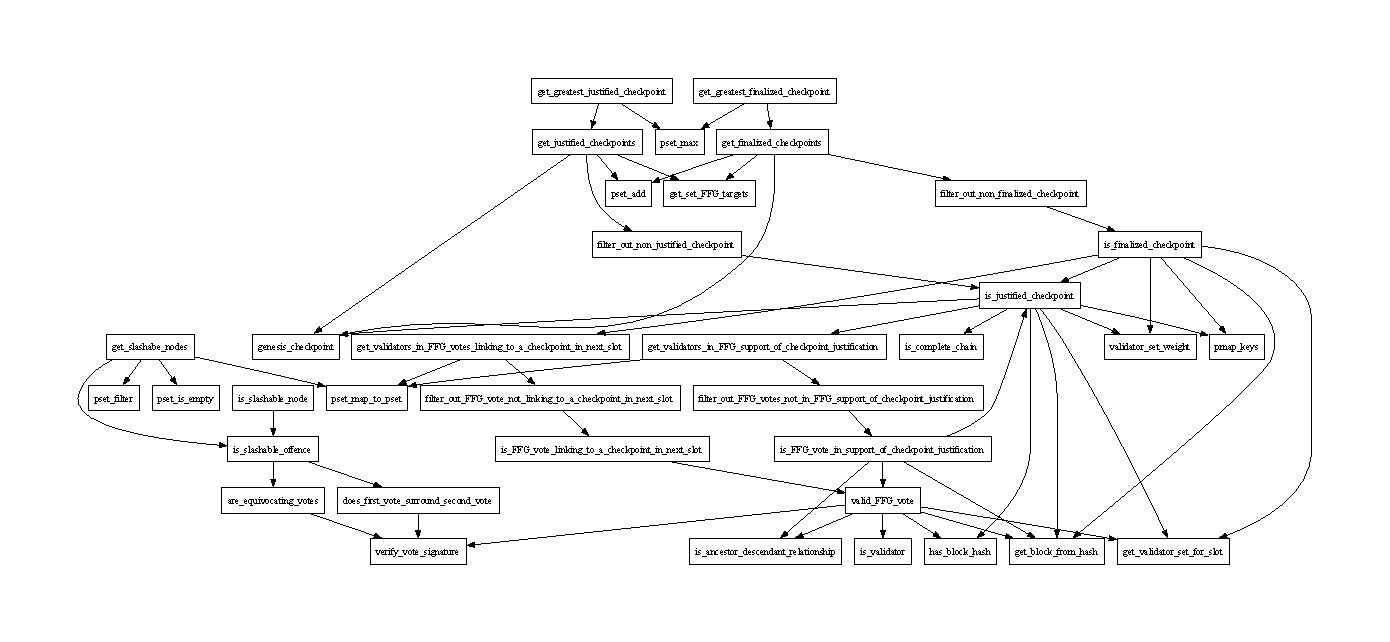
\includegraphics[width=\textwidth,angle=-90]{ffg-callgraph.pdf}
    \caption{The callgraph of the 3SF specification}
    \label{fig:your_label}
\end{figure}

The first specification is obtained by following the principle of least surprise; to the extent that it is possible, without regard to model checking efficiency, we translate Python code to its \tlap{} counterpart with the closest syntax, preserving semantics.

Despite being a programming language and specification language respectively, Python and \tlap{} overlap somewhat in what they can express. 
For instance, both allow us to express sets, and then filter those sets by a given predicate to obtain a different set.
To take a concrete example, observe the definition of $\mathsf{pset\_filter}$ in Figure~\ref{py_filter}.
\begin{figure}
\begin{lstlisting}[language=Python]
def pset_filter(p:Callable[[T1],bool],s: PSet[T1]) -> PSet[T1]:
    r: PSet[T1] = pset()

    for e in s:
        if p(e):
            r = r.add(e)

    return r
\end{lstlisting}
\caption{\textsf{pset\_filter} definition \label{py_filter}}
\end{figure}
%
Notice that, while filter is not one of the built-in operators of the \emph{pyrsistent} library, it is relatively simple to define a filter operator, such that the set returns contains exactly all of the elements of $s$, for which the Boolean predicate $p$ holds true.
In \tlap{}, however, filtering is a language primitive, so if we can translate a python set $s$ to a \tlap{} set $\hat{s}$, and a Python predicate $p$ (of the above type) to a \tlap{} predicate $\hat{p}$, we can translate $\mathsf{pset\_filter}(p, s)$ to $\{ x \in \hat{s}\colon \hat{p}(x) \}$.

We take this idea, and apply it to every definition in the file \texttt{pythonic\_code\_generic.py}, attempting to identify \tlap{}-equivalents (w.r.t. semantics) for each defined function. 
Later on, in milestone 3, we give a formal characterization of all of these equivalencies, in the form of rewriting rules, although for the purposes of this first specification, the entirety of this translation is manual.

Here is an example of a top-level operator, $\mathsf{has\_block\_hash}$\footnote{Python definition available here: \url{https://github.com/saltiniroberto/ssf/blob/ad3ba2c21bc1cd554a870a6e0e4d87040558e129/high_level/common/helpers.py\#L20-L24}}, as it is expressed in \tlap{}:
\begin{lstlisting}[language=tla,columns=fullflexible]
has_block_hash(block_hash, node_state) ==
    block_hash \in DOMAIN node_state.view_blocks
\end{lstlisting}
%
We can see that the original Python implementation calls $\mathsf{pmap\_has}$, which checks whether a key is contained in a given map. In our translation, the map is modeled with a \tlap{} function, which has an associated $\DOMAIN$ set, so we simply check for set membership with the built-in \textsf{\\in}~operator.

Although it is relevant in the process of translation, we do not give explicit rules for the translation of Python language primitives to \tlap{} in general, since attempting to establish those for the full language would vastly exceed the scope of this project. 
Some of these constructs are particularly relevant, and we briefly mention them here:
\paragraph{Assignments and local variables.} There are certain idiosyncrasies to do with the fact that one language is executable, and the other is not. For instance, Python allows for arbitrary variable assignment and reassignment, as well as the introduction of local variables. There are two constructs available in \tlap{} which can be used to express variable assignment:
\begin{itemize}
  \item state-variable update $a' = e$
  \item LET-IN local operator definition $\mathrm{LET}\; v \defeq e \;\mathrm{IN}\; f$
\end{itemize}
to avoid going in to too much detail, it is up to the translator to evaluate which of the two better captures the semantics of the Python code (with, in general, a preference for the LET-IN variant).
\paragraph{Runtime exceptions.} Python code may throw at any time, sometimes in the form of $\mathrm{Require}$-assertions within function definitions. 
In general, this behavior is impossible to replicate without very convoluted \tlap{} code, so we either have to omit those assertions, or return an unspecified value of the correct type if the requirement is not met.

\paragraph{Recursion.} Native \tlap{} supports recursive operators at the language level, but Apalache does not, at the model-checking level. This means that we can translate recursive Python functions as-written in \texttt{Spec 1}, with the knowledge that we will need to remove them in \texttt{Spec 2} to facilitate model checking.


% Milestone 2 - Spec 2
%! TeX root = report.tex

\section{M2: Spec 2: Fold-Based Specification}

\SpecTwo{} addresses some of the limitations inherent in the straightforward
translation of \SpecOne{} from the Python executable specification.

\subsection{Translating Recursive \tlap{} Operators}

The primary goal of \SpecTwo{} is to maintain the semantic structure of
\SpecOne{} while eliminating recursion. In \SpecOne{}, (mutually) recursive
operators model key aspects of protocol behavior, such as the block tree and
block justification. Apalache does not natively support recursive
operators\footnote{\url{https://apalache-mc.org/docs/apalache/principles/recursive.html}},
thus it cannot be used immediately to model-check \SpecOne{}. While the
explicit-state \tlap{} model checker TLC supports recursive operators, it does
not scale to model-checking of this problem.

To resolve this, we reformulate \SpecOne{} into \SpecTwo{}, by substituting
(mutually) recursive constructs with bounded
\texttt{fold}~operations\footnote{In functional programming, \texttt{fold} is a
higher-order function that accepts a combining operation and an iterable data
structure, and applies the operation to each element of the data structure
to compute a single return value. \texttt{fold} is also known as
\texttt{reduce} in some languages.}, which enable the same iterative
computations to be performed in a non-recursive manner. Consider the following
example from \SpecOne{}:

\begin{lstlisting}[language=tla]
RECURSIVE is_ancestor_descendant_relationship(_, _, _)
is_ancestor_descendant_relationship(ancestor, descendant, node_state) ==
    IF ancestor = descendant THEN TRUE
    ELSE IF descendant = node_state.configuration.genesis THEN FALSE
    ELSE
        /\ has_parent(descendant, node_state)
        /\ is_ancestor_descendant_relationship(ancestor, get_parent(descendant, node_state), node_state)
\end{lstlisting}

Its corresponding fold-based formulation is shown below:

\begin{lstlisting}[language=tla]
is_ancestor_descendant_relationship(ancestor, descendant, node_state) ==
    LET FindAncestor(last_block_and_flag, slot) ==
        LET
            last_block == last_block_and_flag[1]
            flag == last_block_and_flag[2]
        IN
        IF flag THEN Pair(last_block, TRUE)
        ELSE IF last_block = node_state.configuration.genesis \/ ~has_parent(last_block, node_state) THEN Pair(last_block, FALSE)
        ELSE LET parent == get_parent(last_block, node_state) IN Pair(parent, parent = ancestor)
    IN
    ApaFoldSeqLeft(FindAncestor, Pair(descendant, descendant = ancestor), MkSeq(MAX_SLOT, LAMBDA i: i))[2]
\end{lstlisting}

\subsection{An Optimization: Flattening Nested Folds}

Initial model checking experiments with \SpecTwo{} revealed significant
challenges related to memory consumption, stemming from the high number of SMT
constraints emitted by Apalache for nested fold operations, which in turn mirror
the complexity of the original nested recursive structures from the Python
specification.

To address these issues, we introduce a manual optimization strategy that
involves flattening nested fold operations. This technique transforms nested
folds into a more manageable structure by employing additional \tlap{} state
variables, similar to memoization or prophecy variables.

For example, we introduce a new \tlap{} state variable
\texttt{PRECOMPUTED\_IS\_ANCESTOR\_DESCENDANT\_RELATIONSHIP} to store
precomputed ancestor-descendant relationships and initialize it with the results
of the fold operation above:

\begin{lstlisting}[language=tla]
LET all_blocks == get_all_blocks(single_node_state) IN
PRECOMPUTED__IS_ANCESTOR_DESCENDANT_RELATIONSHIP =
    [ descendant \in all_blocks |-> { ancestor \in all_blocks : is_ancestor_descendant_relationship(ancestor, descendant, single_node_state) } ]
\end{lstlisting}

Instead of re-evaluating the fold operation each time we need to check if two
blocks are in an ancestor-descendant relationship, we can directly access the
memoized result in a much more efficient map lookup:

\begin{lstlisting}[language=tla]
are_conflicting(chain1, chain2, node_state) ==
    /\ chain1 \notin PRECOMPUTED__is_ancestor_descendant_relationship[chain2]
    /\ chain2 \notin PRECOMPUTED__is_ancestor_descendant_relationship[chain1]
\end{lstlisting}

To further improve our confidence in the correctness of this optimization, we
could produce a proof in TLAPS or run Apalache to show functional equivalence.

\subsection{Checking the Specification}

We can query the specification for reachable protocol states using Apalache.
For example, we can check if a finalized checkpoint exists by writing an
invariant that we expect not to hold. If the invariant below is violated,
Apalache will produce an example of a finalized checkpoint as a counterexample:

\begin{lstlisting}[language=tla]
\* Find a finalized checkpoint (in addition to the genesis checkpoint)
FinalizedCheckpoint_Example ==
    get_finalized_checkpoints(single_node_state) = { genesis_checkpoint(single_node_state) }
\end{lstlisting}

Obviously, we can also check \textit{AccountableSafety} by supplying it as an
invariant to Apalache:

\begin{lstlisting}[language=tla]
AccountableSafety ==
  LET
    finalized_checkpoints == get_finalized_checkpoints(single_node_state)
    finalized_blocks == { get_block_from_hash(checkpoint.block_hash, single_node_state) : checkpoint \in finalized_checkpoints }
    there_are_conflicting_finalized_blocks == \E block1, block2 \in finalized_blocks : are_conflicting(block1, block2, single_node_state)
    slashable_nodes == get_slashable_nodes(single_node_state.view_votes)
  IN there_are_conflicting_finalized_blocks => Cardinality(slashable_nodes) * 3 >= Cardinality(Nodes)
\end{lstlisting}

Table~\ref{tab:spec2} shows the results of model checking \SpecTwo{} with
Apalache. We can see that generating examples of reachable protocol states and
verifying \textit{AccountableSafety} is infeasible due to the high computational
complexity of the specification.

\begin{table}
    \centering
    \begin{tabular}{ll}
        \tbh{Property} & \tbh{Time} \\ \toprule
        Example: conflicting blocks & timeout ($>40$h) \\
        Example: finalized \& conflicting blocks & timeout ($>40$h) \\
        AccountableSafety & timeout ($>40$h) \\ \bottomrule
    \end{tabular}
    \caption{Model checking \SpecTwo{} with Apalache.}\label{tab:spec2}
\end{table}

These results are not surprising -- the solver has to consider both reachability
properties for all possible block graphs, and all possible FFG voting scenarios
on top of these graphs. To further evaluate \SpecTwo{}, we fix the block graph
-- this way the solver only has to reason about voting. We encode three example
block graphs: a single, linear chain (\texttt{SingleChain}), a minimal forked
chain of three blocks (\texttt{ShortFork}), and a forest of disconnected chains
(\texttt{Forest}). Table~\ref{tab:spec2_fixed} shows the results of model
checking \SpecTwo{} for these fixed block graphs.

\begin{table}
    \centering
    \begin{tabular}{llr}
      \tbh{Property} & \tbh{Block graph} & \tbh{Time} \\ \toprule
      Example: conflicting blocks & \texttt{SingleChain} & 1 min 3 sec \\
      Example: conflicting blocks & \texttt{ShortFork} & 52 sec \\
      Example: conflicting blocks & \texttt{Forest} & 2 min 21 sec \\ \midrule
      Example: fin.\ \& confl.\ blocks & \texttt{SingleChain} & 1 min 5
      sec \\
      Example: fin.\ \& confl.\ blocks & \texttt{ShortFork} & 10 hours
      49 min 47 sec \\
      Example: fin.\ \& confl.\ blocks & \texttt{Forest} & timeout
      ($>40$h) \\ \midrule
      AccountableSafety & \texttt{SingleChain} & 1 min 13 sec \\
      AccountableSafety & \texttt{ShortFork} & timeout ($>40$h) \\
      AccountableSafety & \texttt{Forest} & timeout ($>40$h) \\ \bottomrule
    \end{tabular}
    \caption{Model checking \SpecTwo{} for fixed block
    graphs.}\label{tab:spec2_fixed}
\end{table}

We can see that the solver can handle the single chain block graph (where
\textit{AccountableSafety} trivially holds due to absence of conflicting
blocks), but struggles with the more complex scenarios even when given a fixed
block graph. This suggests that the complexity inherent in the specification is
due to the high combinatorial complexity of voting scenarios, rather than just
the block graph.

\subsection{Discussion}~\footnote{\color{red}TODO: perhaps move this to a general
discussion section?} Applying translation rules to obtain checkable
specifications from other artifacts can provide a useful starting point.
However, such translation are also likely to introduce unwanted
inefficiencies. Translation rules cannot account for the nuances of the specific
context, which can lead to suboptimal performance. Consequently, leveraging
human ingenuity to develop specifications from the outset can be more effective.
When relying on translated specifications, it becomes crucial to conduct
manual optimizations to ensure efficiency.


% Milestone 4 - Specs 3-4

%! TeX root = report.tex

\section{M4: Spec 3}

\paragraph{Motivation.} In the course of writing \texttt{Spec 2}, we realized
that the executable Python specification was essentially sequential. In other
words, even though the 3SF algorithm is distributed, its Python
specification as well as \texttt{Spec 1} and \texttt{Spec 2} were encoding the
execution history in a specification state.

Since \tlap{} is designed for reasoning about state machines, Apalache is tuned
towards incremental model checking of the executions. For instance, if a state
machine is composed of $n$ kinds of state-transitions (called actions), that
is, $\mathit{Next} = A_1 \vee \dots \vee A_N$, then model checker tries to find
a violation to a state invariant~$\textit{Inv}$ by assuming that a single
symbolic transition $A_i$ took place. If there is no violation, that instance
of the invariant~$\textit{Inv}$ can be discarded. By doing so, the model
checker reduces the number of constraints for the SMT solver to process.  The
same applies to checking an inductive invariant. When there is no such a
decomposition of $\mathit{Next}$, the model checker produces harder problems
for SMT\@.

\paragraph{Introducing a state machine.} Having this observation in mind, we
introduced \texttt{Spec 3} that incrementally builds the following data structures:

\begin{itemize}

    \item The set of proposed blocks, and the graph containing these blocks,
        called $\textit{blocks}$ and $\textit{graph}$, respectively.

    \item The ancestor-descendant relation, called
        $\textit{block\_graph\_closure}$.

    \item The announced FFG votes and the validators' votes on them, called
        $\textit{ffg\_votes}$ and $\textit{votes}$, respectively.

    \item The set of justified checkpoints that is computed as the greatest
        fixpoint, called $\textit{justified\_checkpoints}$.

\end{itemize}

Perhaps, the most essential part of the specification is show in
Figure~\ref{fig:abstract-ffg-cast-votes}. It represents an abstract
state-transition that corresponds to a subset of validators sending votes for
the same FFG vote. The most interesting part of this transition can be seen in
the last lines: Instead of directly computing the set of justified checkpoints
in the current state, we just ``guess'' it and impose the required constraints
on this set. Mathematically, $\textit{justified\_checkpoints}$ is the greatest
fixpoint among the checkpoints that satisfy the predicate
$\textit{IsJustified}$.


\begin{figure}
    \centering
    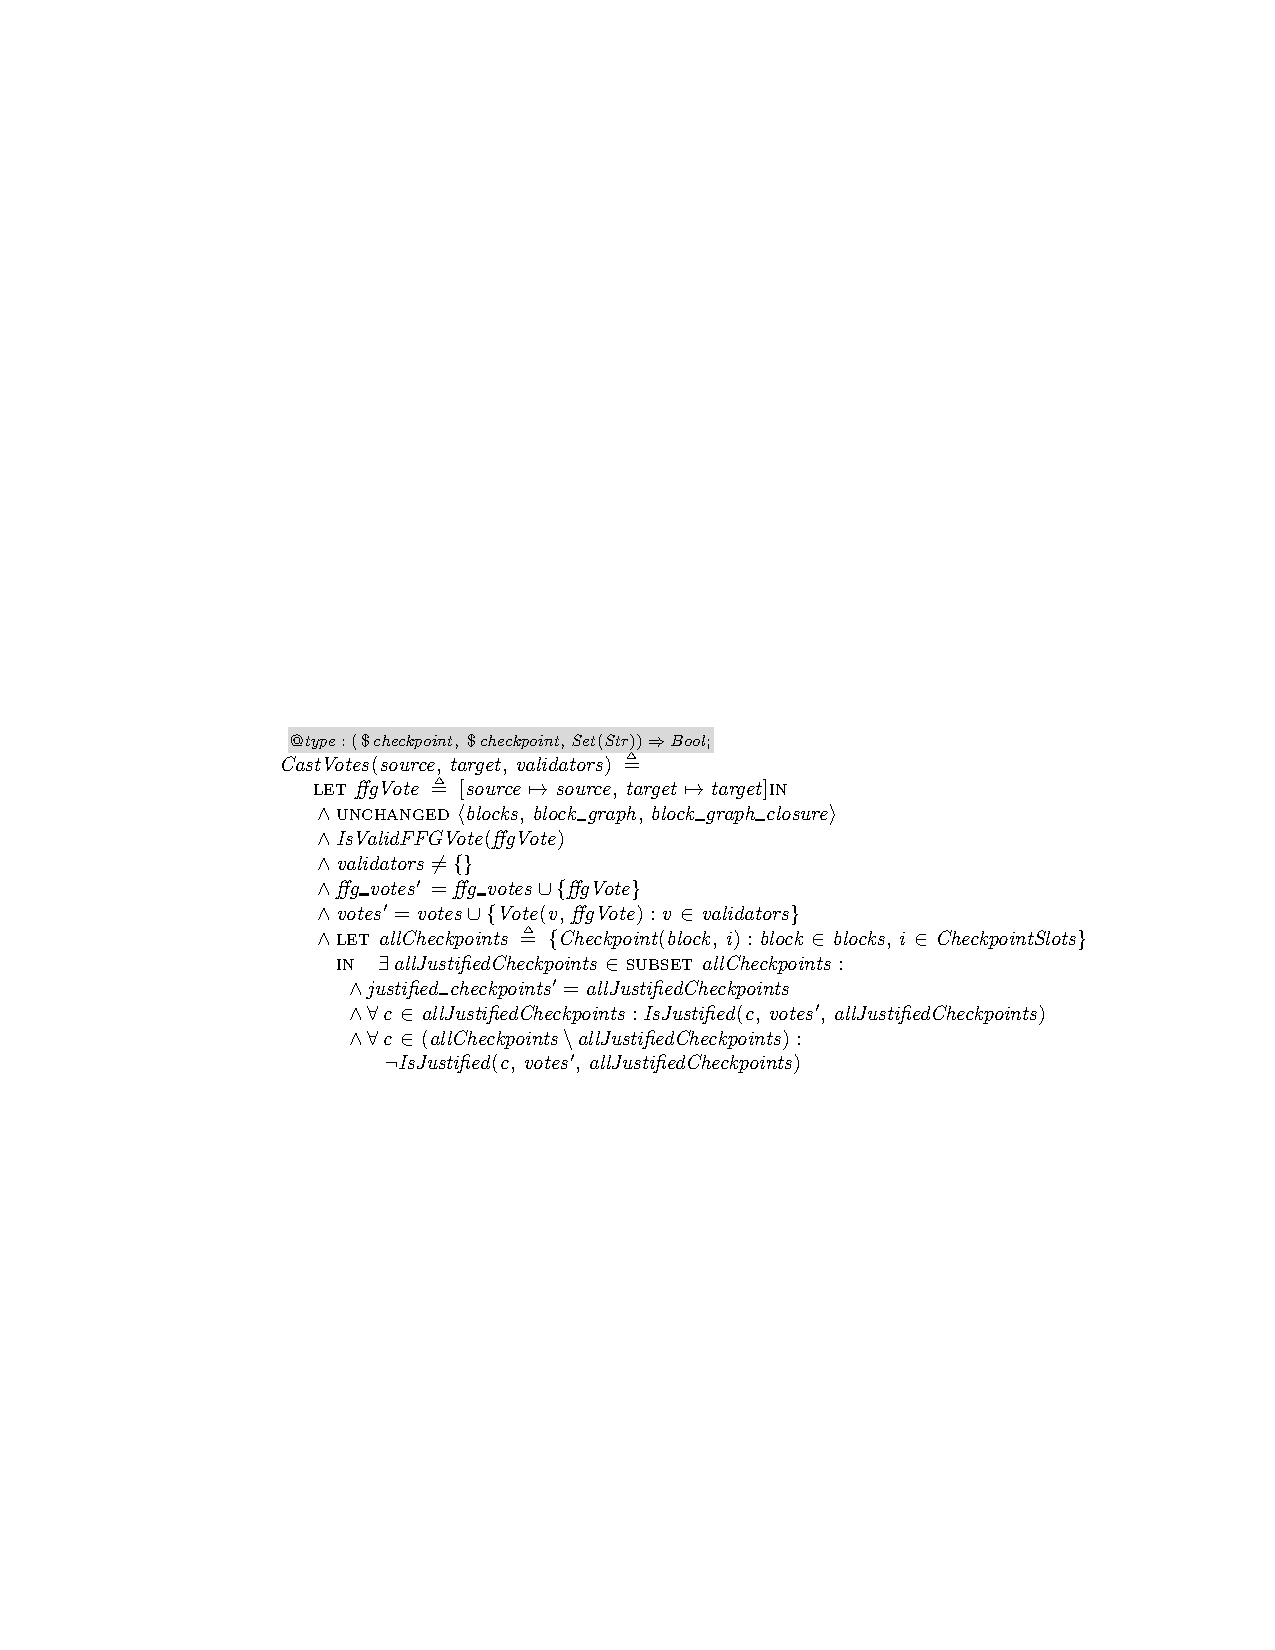
\includegraphics[width=\textwidth]{images/abstract-ffg-cast-votes.pdf}  % Include the PDF file
    \caption{A state-transition that casts votes}\label{fig:abstract-ffg-cast-votes}
\end{figure}

Figure~\ref{fig:abstract-ffg-next} shows the transition predicate of the
specification. It just non-deterministically chooses the inputs to
$\textit{ProposeBlock}$ or $\textit{CastVotes}$ and fires one of those two
actions.

\begin{figure}
    \centering
    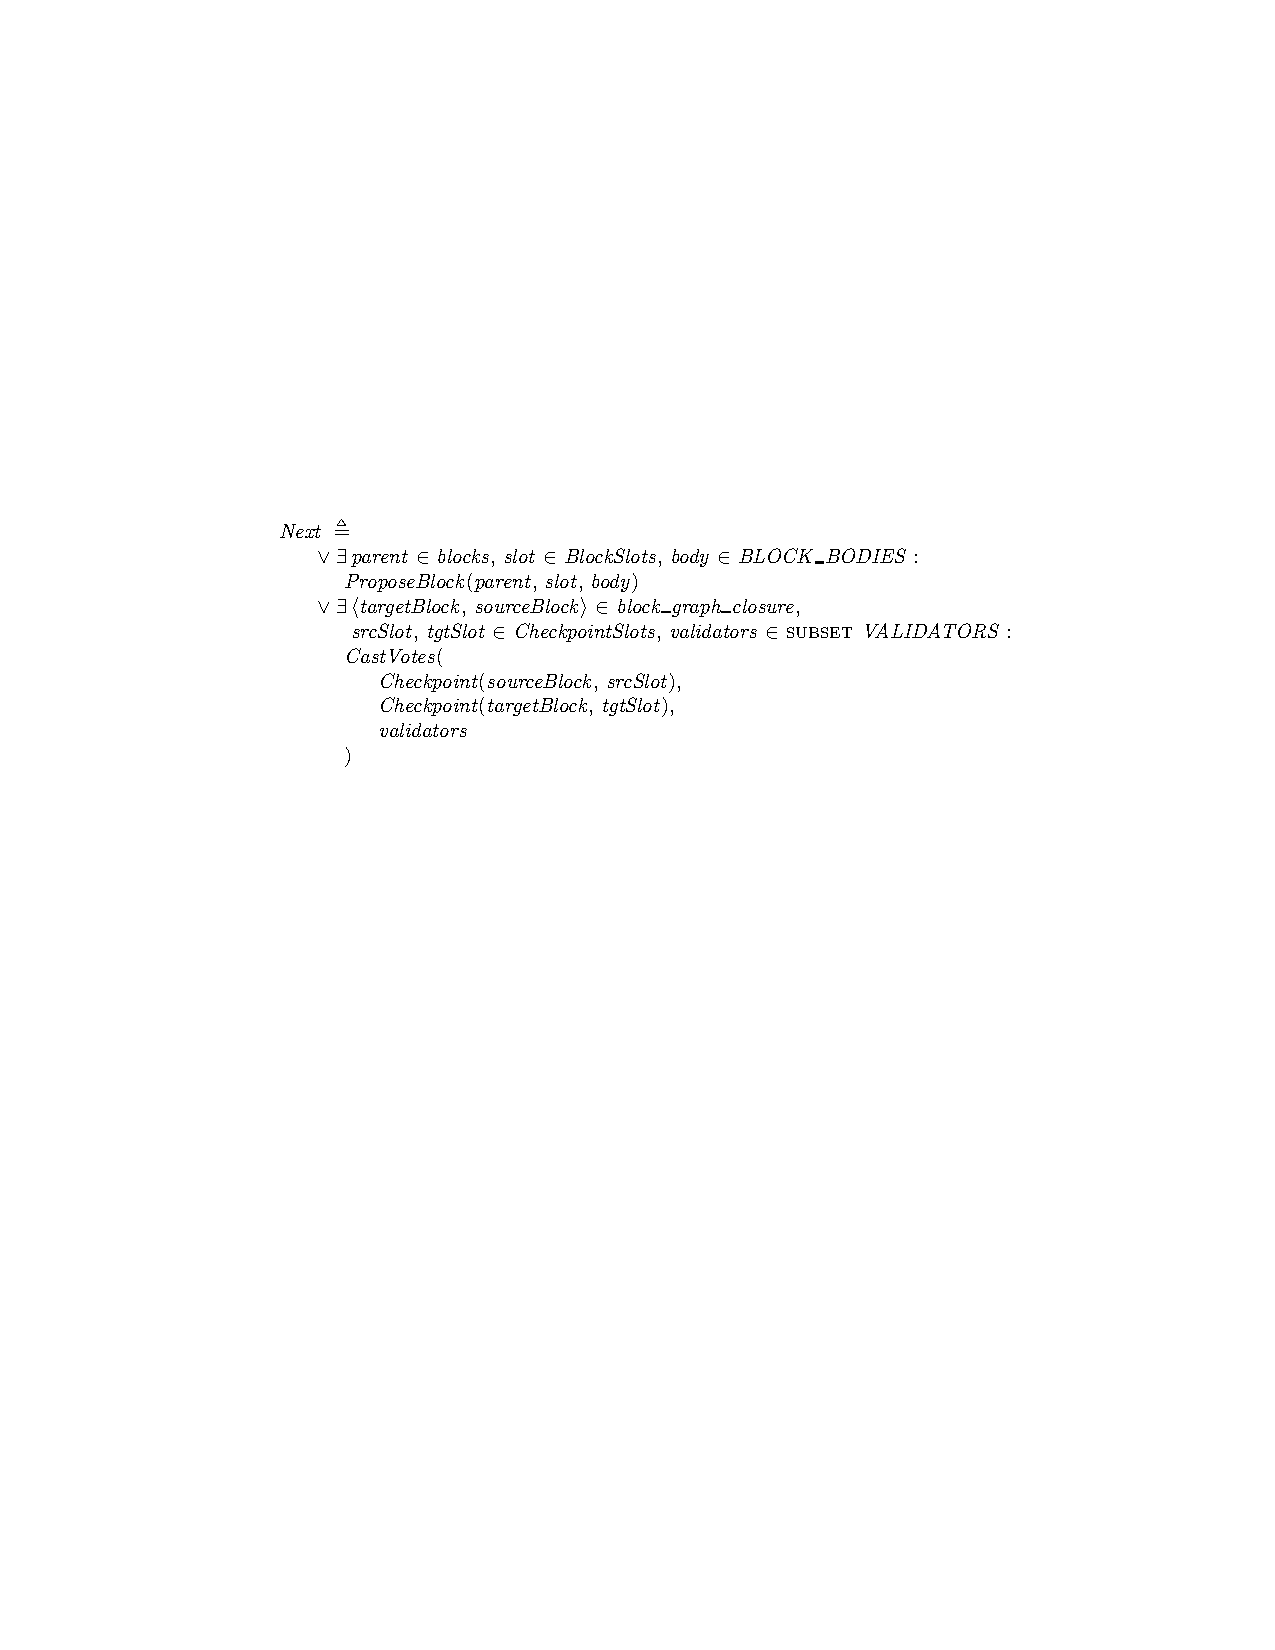
\includegraphics[width=\textwidth]{images/abstract-ffg-next.pdf}  % Include the PDF file
    \caption{The transition predicate of Spec 3}\label{fig:abstract-ffg-next}
\end{figure}

\paragraph{Model checking experiments.} We have conducted model checking
experiments with this specification. They are summarized in
Table~\ref{tab:abstract-ffg-mc}.

\begin{table}
    \centering
    \begin{tabular}{lr}
        \tbh{State invariant} & \tbh{Command} & \tbh{Time} \\ \toprule
        $\textit{ExistsJustifiedNonGenesisInv}$ & \texttt{check} & 5s \\ \midrule
        $\textit{ExistTwoFinalizedConflictingBlocks}$ & \texttt{check} & NNN \\ \midrule
        $\textit{AccountableSafety}$ & \texttt{simulate} & NNN \\ \midrule
        $\textit{AccountableSafety}$ & \texttt{check} & NNN \\ \bottomrule
    \end{tabular}
    \caption{Model checking experiments with Spec 3}\label{tab:abstract-ffg-mc}
\end{table}


%! TeX root = report.tex

\section{Spec 4: Two chains in \tlap{}}\label{sec:spec4}

We obtain this specification by preserving the vote and checkpoint behavior from \SpecThree{}, but we restrict the block-graph to exactly two chains, which are allowed to fork, i.e., they always share a common prefix.
To this end, we restrict block bodies of the two chains as follows:
\begin{enumerate}
	\item Block bodies on the first chain have nonnegative sequential integer numbers starting from 0 (genesis), e.g. $0, 1, 2,3, 4$.
	\item Block bodies on the second chain are the same as the ones on the first chain \emph{up to the fork point}, after which they change sign, but otherwise maintain their sequence in absolute value terms, e.g. $0, 1,2,-3,-4$.
\end{enumerate}

The aim of this encoding is to decrease complexity for the SMT solver, since it simplifies block graph ancestry and closure reasoning significantly (e.g. we can check whether one block is an ancestor of another by simply comparing block body integer values), while preserving the behavior which arises from voting on checkpoint justification.

\subsection{Inductive Invariant}\label{sec:spec4-indinv}

This specification defines an inductive invariant \textit{IndInv}. Recall, an inductive invariant satisfies the following two conditions, assuming we have an initial-state predicate \textit{Init}, and transition predicate \textit{Next}:
\begin{enumerate}
	\item It is implied by the initial state: $\mathit{Init} \Rightarrow \mathit{IndInv}$
	\item It is preserved by the transition predicate: $\mathit{IndInv} \land \mathit{Next} \Rightarrow \mathit{IndInv}$
\end{enumerate}
Because of this characterization, inductive invariants lend themselves especially nicely to bounded symbolic model checking; with Apalache, one can prove (or disprove) an inductive invariant by running two queries of depth at most 1, corresponding to the above properties.
If no violation is found, we are assured that \textit{IndInv} holds in all possible reachable states.
Since our goal is ultimately to prove or disprove \textit{AccountableSafety}, we can additionally prove $\mathit{IndInv} \Rightarrow \mathit{AccountableSafety}$.

The challenge, typically, is that inductive invariants are more difficult to write, compared to state invariants.
They are usually composed of several lemmas, i.e. properties that we are less interested in on their own, but which are crucial in establishing property (2.).

As we explain below, the inductive invariant introduced in \SpecFour{} mainly contains of two sets of lemmas, one for characterizing the chain-fork scenarios, and a second one for characterizing justified checkpoints, shown in Figure~\ref{figFork} and Figure~\ref{figJC} respectively.

\begin{figure}
  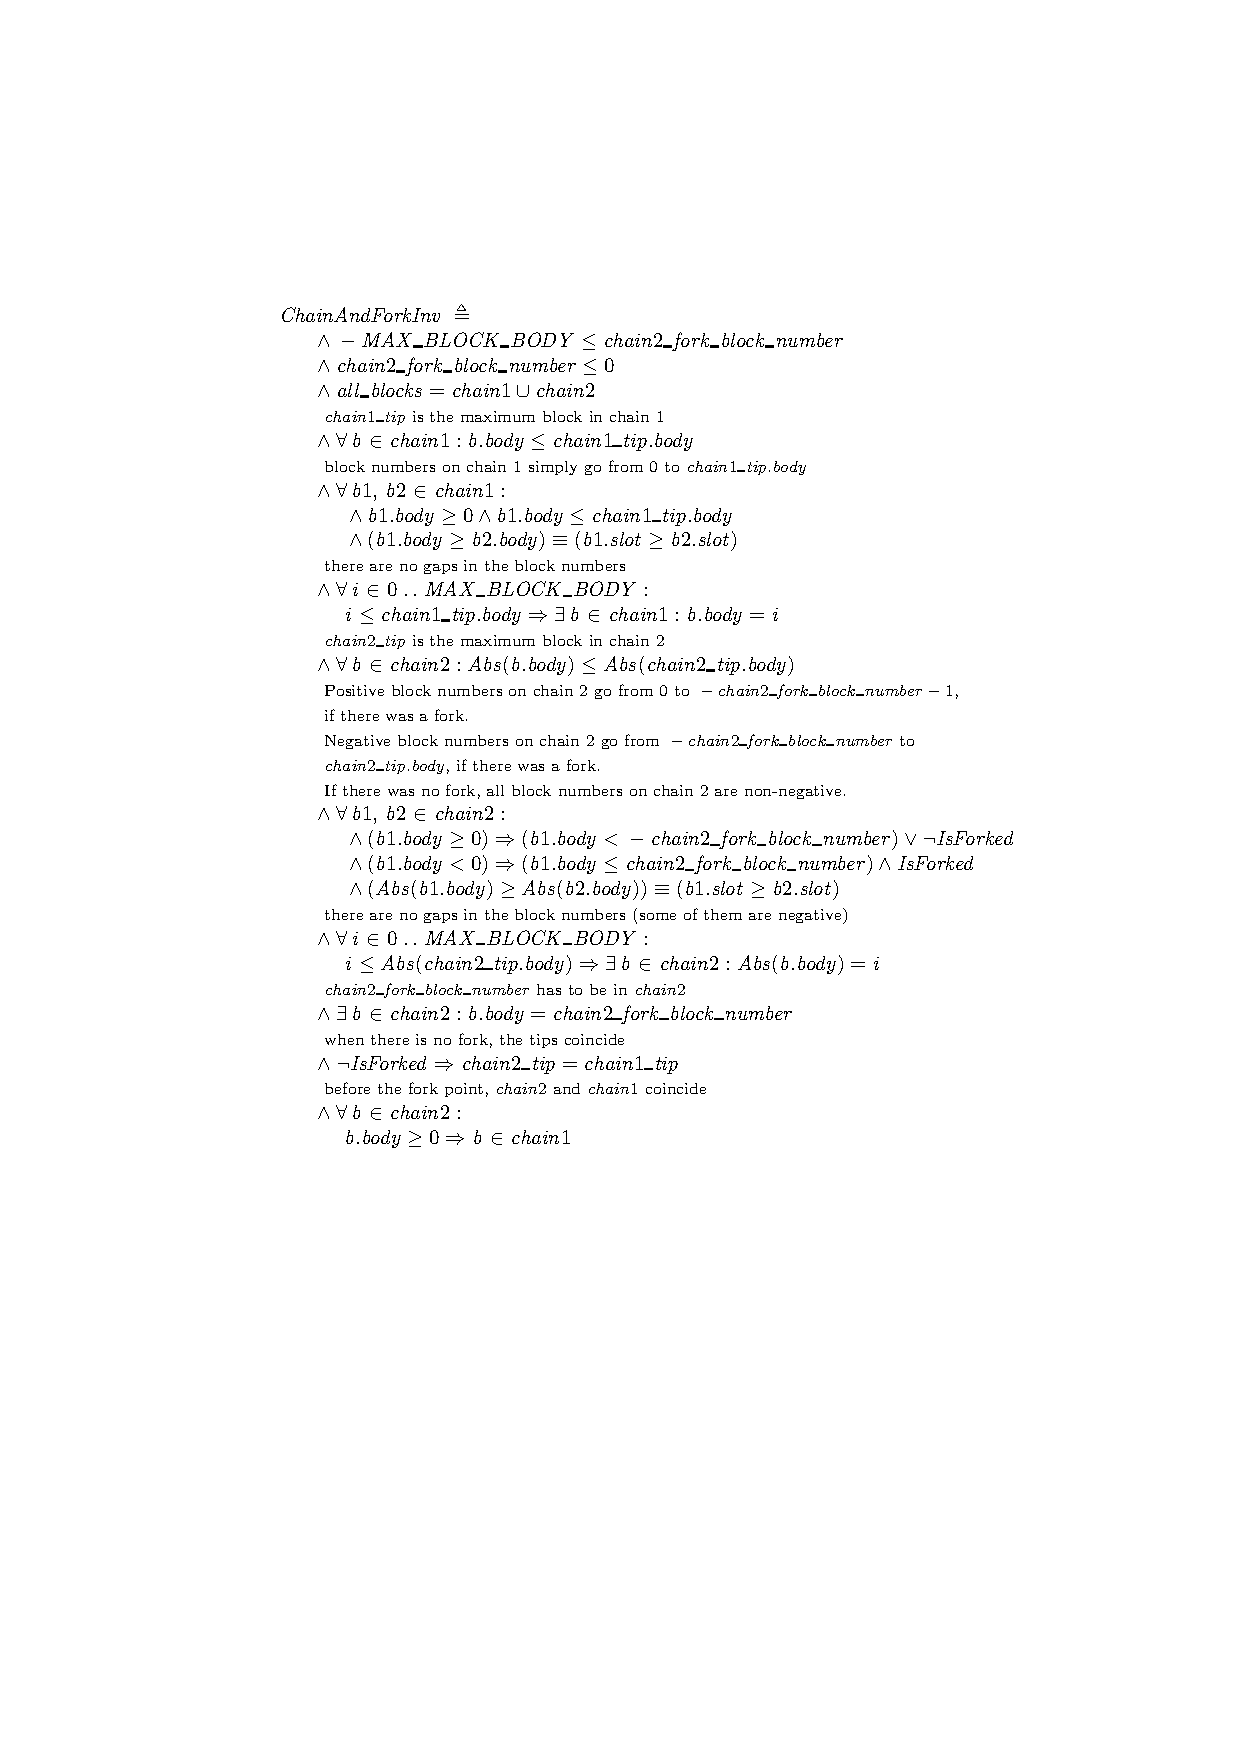
\includegraphics[width=\textwidth]{images/chain-and-fork-inv.pdf}
  \caption{Chain and forking lemmas in \textit{IndInv}}\label{figFork}
\end{figure}

\begin{figure}
  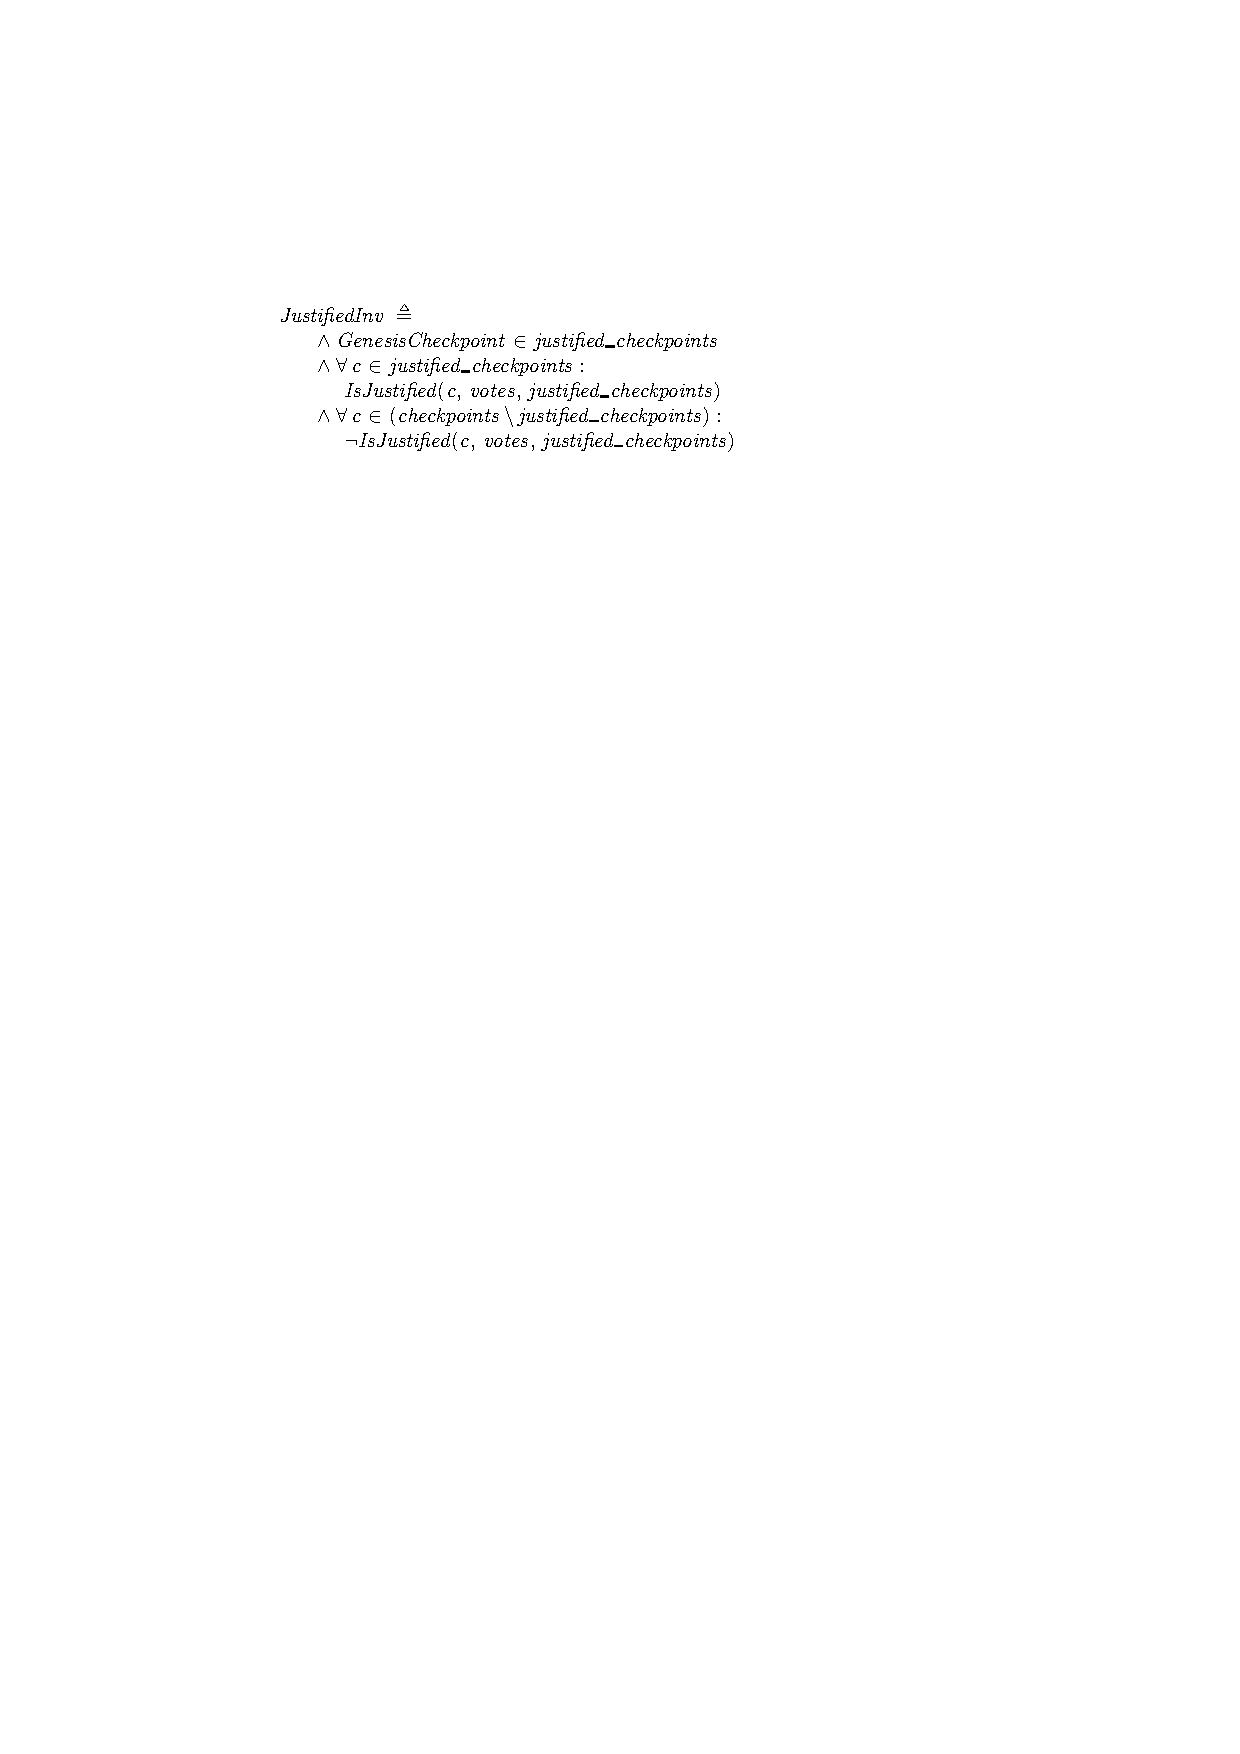
\includegraphics[width=\textwidth]{images/justified-inv.pdf}
  \caption{Justified checkpoint lemmas in \textit{IndInv}}\label{figJC}
\end{figure}

Since we represent a fork by means of a sign-change on block numbers, we have to specify that their absolute values are contiguous, that the chains coincide in the absence of a fork, as well as on the pre-fork prefix, and that both chains are monotone w.r.t. block numbers after the fork point.
Additionally, we require validity predicates for the vote set and checkpoints, as well as a precise characterization of the set of justified checkpoints. The latter merits further discussion.

\paragraph{Justified checkpoints.} To accurately describe the set of all justified checkpoints, we require two constraints:
\begin{enumerate}
	\item Consistency: Every checkpoint in the set is justified, and 
	\item Completeness: Every justified checkpoint belongs to the set.
\end{enumerate}
It is worth noting that both of these properties are required for an inductive invariant; if we don't specify consistency, the solver can trivially infer that the set contains all possible checkpoints, and that all checkpoints are finalized, which leads to bogus counterexamples to \textit{AccountableSafety}.
On the other hand, if we don't specify completeness, the solver can trivially infer that the set of justified checkpoints is empty (or contains exactly the genesis checkpoint). This leads us to be unable to detect real violations of \textit{AccountableSafety}, since we can never observe conflicting finalized checkpoints, even when the votes cast necessitate their existence.

This is critical, because including both constraints places a heavy burden on the solver. No matter how we define the justification predicate, it will inevitably appear in both positive and negative form, forcing the solver to contend with both quantifier alternations and double universal quantification, both of which are known to be hard.
Fundamentally, this demonstrates the intrinsic complexity of the problem itself, regardless of the particular characterization of justified sets in \tlap{}.

\subsection{Model checking experiments}

TODO\footnote{IK: describe the further optimizations}


%! TeX root = report.tex

\section{Spec 4c in SMT using Finite Sets \& Cardinalities}

In addition to \SpecFour{}, we have developed a manual encoding of the 3SF
protocol in SMT, directly utilizing the CVC5
solver~\cite{DBLP:conf/tacas/BarbosaBBKLMMMN22}. Following the same
structure as \SpecFour{}, the encoding captures the key components of the 3SF
protocol, including checkpoints, FFG votes, justified and finalized blocks,
and slashing conditions.
To model finite sets and cardinalities, we use the non-standard SMT theory of
sets and cardinalities~\cite{DBLP:journals/lmcs/BansalBRT18} provided by CVC5.

In contrast to the \tlap{}-based \SpecFour{}, we manually encode the protocol
directly as SMT-LIB constraints. At the cost of using a lower-level language and
requiring a specialized solver, this has the following advantages:
\begin{itemize}
  \item The manual encoding is more succinct than the SMT encoding produced by
    Apalache from \tlap{}.
  \item SMT-LIB supports recursive functions, which allows us to express the
    recursion inherent to the 3SF protocol more naturally.
\end{itemize}

\subsection{Modeling}
The SMT spec explicitly introduces hashes, checkpoints and nodes as atoms over
finite domains. In contrast, votes are modeled as any possible combination
of a source and target checkpoint and a sending node:

\begin{lstlisting}[language=smt]
(declare-datatype Hash ((Hash1) (Hash2) (Hash3)))
(declare-datatype Checkpoint ((C1) (C2) (C3) (C4) (C5)))
(declare-datatype Node ((Alice) (Bob) (Charlie) (David)))
(declare-datatype Vote ((Vote (source Checkpoint) (target Checkpoint) (sender Node))))
\end{lstlisting}

To remain within the decidable SMT fragment, we have to model unbounded data
using functions. For example, we model the slot number of a block as a function
from block hashes to integers:

\begin{lstlisting}[language=smt]
(declare-fun slot (Hash) Int)
; genesis' slot is 0
(assert (= (slot genesis) 0))
; slots are increasing from parent to child
(assert (forall ((h Hash)) (=> (not (= h genesis)) (> (slot h) (slot (parent_of h))))))
\end{lstlisting}

We encode all protocol rules as declarative constraints in the SMT model. For
example, the constraint that a checkpoint is justified if and only if there is
a supermajority of validators that cast a justifying vote from an already
justified checkpoint is encoded as follows:

\begin{lstlisting}[language=smt]
(declare-const justified_checkpoints (Set Checkpoint))
(assert (= justified_checkpoints (set.comprehension ((c Checkpoint))
  (or
    ; L3: genesis is justified
    (= c genesis_checkpoint)
    ; L4: there is a quorum of validators that cast a vote from a justified checkpoint to c
    (>= (* 3 (set.card (set.comprehension ((node Node))
        (exists ((vote Vote)) (and
          ; L4+5: vote is a valid vote cast by node
          (set.member vote votes)
          (= (sender vote) node)
          ; L6: the source of the vote is justified
          (set.member (source vote) justified_checkpoints)
          ; L7: there is a chain source.block ->* checkpoint.block ->* target.block
          (and
            (set.member (tuple (checkpoint_block (source vote)) (checkpoint_block c)) ancestor_descendant_relationship)
            (set.member (tuple (checkpoint_block c) (checkpoint_block (target vote))) ancestor_descendant_relationship)
          )
          ; L8: the target checkpoint slot is the same as the checkpoint's
          (= (checkpoint_slot (target vote)) (checkpoint_slot c))
        ))
        node
      )))
      (* 2 N)
    )
  )
  c
)))
\end{lstlisting}

%! TeX root = report.tex

\section{Spec 4 -- Alloy}

TODO\footnote{IK: describe}




% Milestone 3 - Translation rules
%! TeX root = report.tex

\section{Translating Python specifications to \tlap{}}\label{section3}

In this section, we present our results on translating a subset of Python that
is used to write executable specifications in the projects such as
\texttt{ssf-mc}\footnote{\url{https://github.com/saltiniroberto/ssf}}. Since we
have done the translation by hand, our rules are currently formalized on paper.
Additionally, in case of non-trivial rules, we give correctness proofs.

Since the Python subset uses the package $\texttt{pyrsistent}$, we assume that
the expressions are typed according to the package types, which can be found in
the $\texttt{typing}$ module. In the following, given a Pyrsistent type $\tau$,
we will denote its corresponding type in the Apalache type
system~1.2\footnote{\url{https://apalache-mc.org/docs/adr/002adr-types.html}}
with $\htau$. Table~\ref{tab:types} shows the types mapping.

\begin{table}[!h]
    \centering
    \begin{tabular}{cc}
        \tbh{Pyrsistent type} & \tbh{Apalache type}
            \\\toprule
        bool & Bool \\\midrule
        int & Int \\\midrule
        str & Str \\\midrule
        $\PSet[\tau]$ & $\Set(\htau)$ \\\midrule
        $\PVec[\tau]$ & $\List(\htau) \defeq \{ es\colon \Seq(\htau) \}$ \\\midrule
        $\PMap[\tau_1, \tau_2]$ & $\htau_1 \rightarrow \htau_2$ \\\midrule
        $\Callable[[\tau_1], \tau_2]$ & $\tau_1 \Rightarrow \tau_2$ \\\midrule
    \end{tabular}
    \caption{Mapping the Pyrsistent
             types to Apalache types}\label{tab:types}
\end{table}

Note that instead of using the standard type $\Seq(\htau)$ of \tlap{}, which
represents 1-indexed sequences, we use an alternative module
\texttt{Lists}\footnote{\url{https://github.com/konnov/tlaki/blob/main/src/Lists.tla}},
which represents 0-indexed sequences. To that end, we introduce the type
notation:

\[ \List(\htau) \coloneqq \{ es\colon \Seq(\htau) \} \]

The translation rules can be easily adapted to~$\Seq(\htau)$ instead
of~$\List(\htau)$.

\subsection{Translation rules}

We will be using the \href{https://github.com/konnov/tlaki/blob/main/src/Lists.tla}{$\texttt{Lists}$} module, in lieu of $\texttt{Sequences}$, to better match the 0-indexing convention of Python. To that end, we introduce the type notation:
\[
\List(\htau) \coloneqq \{ es\colon \Seq(\htau) \}
\]
that is, the instantiation of the $\texttt{list}$ alias defined in $\texttt{Lists.tla}$ with the concrete type $\hat{t}$.

\subsubsection{Singleton vector}
\href{https://github.com/saltiniroberto/ssf/blob/7ea6e18093d9da3154b4e396dd435549f687e6b9/high_level/common/pythonic_code_generic.py#L15-L16}{Source}.


%     a: t
%   ==========   pvector_of_one_element(a) 
%     e: t^
% ==========================================
%         List(<< e >>) : List(t^)

\begin{mathpar}
    \inferrule*[right=(\textsc{Vec})]
    {
        \inferrule{a\colon \tau}{e \colon \htau}
        \\
        \mathrm{pvector\_of\_one\_element}(a)
    }{
        \List(\tup{e})\colon \List(\htau)
    }
\end{mathpar}
A singleton Python vector is translated to a single-element list, and annotated as such.

\subsubsection{Vector concatenation}
\href{https://github.com/saltiniroberto/ssf/blob/7ea6e18093d9da3154b4e396dd435549f687e6b9/high_level/common/pythonic_code_generic.py#L19-L20}{Source}.


%    a: PVec[t]        b: PVec[t]
%  ===============   ===============   pvector_concat(a, b) 
%    e: List(t^)       f: List(t^)
% ============================================================
%                  Concat(e,f) : List(t^)

\begin{mathpar}
    \inferrule*[right=(\textsc{Concat})]
    {
        \inferrule{a\colon \PVec[\tau]}{e \colon \List(\htau)}
        \\
        \inferrule{b\colon \PVec[\tau]}{f \colon \List(\htau)}
        \\
        \mathrm{pvector\_concat}(a, b)
    }{
        \Concat(e,f) \colon \List(\htau)
    }
\end{mathpar}
Vector concatenation is translated to the list concatenation.

\subsubsection{Set sequentialization}
\href{https://github.com/saltiniroberto/ssf/blob/7ea6e18093d9da3154b4e396dd435549f687e6b9/high_level/common/pythonic_code_generic.py#L23-L24}{Source}.


%          a: PSet[t]         
%        ==============   from_set_to_pvector(a) 
%          e: Set(t^)       
% ======================================================
%   ApaFoldSet( Push, List(<<>>: Seq(t^)), e ) : List(t^)

\begin{mathpar}
    \inferrule*[right=(\textsc{SetToVec})]
    {
        \inferrule{a\colon \PSet[\tau]}{e \colon \Set(\htau)}
        \\
        s \coloneqq \tup{}\colon \Seq(\htau)
        \\
        \mathrm{from\_set\_to\_pvector}(a)
    }{
        \ApaFoldSet( \Push, \List(s), e ) \colon \List(\htau)
    }
\end{mathpar}
We use fold, to create a sequence (in some order) from the set.

\subsubsection{ Empty set}
\href{https://github.com/saltiniroberto/ssf/blob/7ea6e18093d9da3154b4e396dd435549f687e6b9/high_level/common/pythonic_code_generic.py#L27-L28}{Source}.


%   pset_get_empty : PSet[t]
% ============================
%        {} : Set(t^)

\begin{mathpar}
    \inferrule*[right=(\textsc{EmptySet})]
    {
        \mathrm{pset\_get\_empty}() \colon \PSet[t]
    }{
        \{\} \colon \Set(\htau)
    }
\end{mathpar}
The only relevant part here is that we need a type annotation on the Python side to correctly annotate the empty set in \tlap{}.

\subsubsection{ Set union}
\href{https://github.com/saltiniroberto/ssf/blob/7ea6e18093d9da3154b4e396dd435549f687e6b9/high_level/common/pythonic_code_generic.py#L31-L32}{Source}.


%     a: PSet[t]       b: PSet[t]
%   ==============   ==============   pset_merge(a, b) 
%     e: Set(t^)       f: Set(t^)
% ======================================================
%                 e \cup f : Set(t^)

\begin{mathpar}
    \inferrule*[right=(\textsc{Union})]
    {
        \inferrule{a\colon \PSet[\tau]}{e \colon \Set(\htau)}
        \\
        \inferrule{b\colon \PSet[\tau]}{f \colon \Set(\htau)}
        \\
        \mathrm{pset\_merge}(a, b)
    }{
        e \cup f \colon \Set(\htau)
    }
\end{mathpar}
Set union is translated to the \tlap{} native set union.

\subsubsection{ Set flattening}
\href{https://github.com/saltiniroberto/ssf/blob/7ea6e18093d9da3154b4e396dd435549f687e6b9/high_level/common/pythonic_code_generic.py#L35-L36}{Source}.


%          a: PSet[PSet[t]]         
%        ====================   pset_merge_flatten(a) 
%          e: Set(Set(t^))       
% =====================================================
%                 UNION e : Set(t^)

\begin{mathpar}
    \inferrule*[right=(\textsc{BigUnion})]
    {
        \inferrule{ a\colon \PSet[\PSet[\tau]]}{e \colon \Set(\Set(\htau))}
        \\
        \mathrm{pset\_merge\_flatten}(a)
    }{
        \UNION e \colon \Set(\htau)
    }
\end{mathpar}
Set flattening is translated to the \tlap{} native big $\UNION$.

\subsubsection{Set intersection}
\href{https://github.com/saltiniroberto/ssf/blob/7ea6e18093d9da3154b4e396dd435549f687e6b9/high_level/common/pythonic_code_generic.py#L42-L43}{Source}.


%     a: PSet[t]       b: PSet[t]
%   ==============   ==============   pset_intersection(a, b) 
%     e: Set(t^)       f: Set(t^)
% =============================================================
%                    e \cap f : Set(t^)

\begin{mathpar}
    \inferrule*[right=(\textsc{Intersection})]
    {
        \inferrule{a\colon \PSet[\tau]}{e \colon \Set(\htau)}
        \\
        \inferrule{b\colon \PSet[\tau]}{f \colon \Set(\htau)}
        \\
        \mathrm{pset\_intersection}(a, b)
    }{
        e \cap f \colon \Set(\htau)
    }
\end{mathpar}
Set intersection is translated to the \tlap{} native set intersection.

\subsubsection{Set difference}
\href{https://github.com/saltiniroberto/ssf/blob/7ea6e18093d9da3154b4e396dd435549f687e6b9/high_level/common/pythonic_code_generic.py#L46-L47}{Source}.


%     a: PSet[t]       b: PSet[t]
%   ==============   ==============   pset_difference(a, b) 
%     e: Set(t^)       f: Set(t^)
% ===========================================================
%                       e \ f : Set(t^)

\begin{mathpar}
    \inferrule*[right=(\textsc{SetDiff})]
    {
        \inferrule{a\colon \PSet[\tau]}{e \colon \Set(\htau)}
        \\
        \inferrule{b\colon \PSet[\tau]}{f \colon \Set(\htau)}
        \\
        \mathrm{pset\_difference}(a, b)
    }{
        e \setminus f \colon \Set(\htau)
    }
\end{mathpar}
Set difference is translated to the \tlap{} native set difference.

\subsubsection{Singleton set}
\href{https://github.com/saltiniroberto/ssf/blob/7ea6e18093d9da3154b4e396dd435549f687e6b9/high_level/common/pythonic_code_generic.py#L50-L51}{Source}.

%     a: t
%   =========   pset_get_singleton(a) 
%     e: t^
% =====================================
%            { e } : Set(t^)

\begin{mathpar}
    \inferrule*[right=(\textsc{Singleton})]
    {
        \inferrule{a\colon \tau}{e \colon \htau}
        \\
        \mathrm{pset\_get\_singleton}(a)
    }{
        \{e\} \colon \Set(\htau)
    }
\end{mathpar}
A singleton Python set is translated to a \tlap{} native single-element set.

\subsubsection{Set extension}
\href{https://github.com/saltiniroberto/ssf/blob/7ea6e18093d9da3154b4e396dd435549f687e6b9/high_level/common/pythonic_code_generic.py#L54-L55}{Source}.


%     a: PSet[t]       b: t
%   ==============   =========  pset_add(a, b) 
%     e: Set(t^)       f: t^
% ==============================================
%             e \cup { f } : Set(t^) 

\begin{mathpar}
    \inferrule*[right=(\textsc{SetExt})]
    {
        \inferrule{a\colon \PSet[\tau]}{e \colon \Set(\htau)}
        \\
        \inferrule{b\colon \tau}{f \colon \htau}
        \\
        \mathrm{pset\_add}(a, b)
    }{
        e \cup \{f\} \colon \Set(\htau)
    }
\end{mathpar}
A set extension is translated to a combination of union and singleton-set construction. Semantically, this is the equivalence
\[
\mathrm{pset\_add}(a,b) = \mathrm{pset\_merge}(a, \mathrm{pset\_get\_singleton}(b))
\]

\subsubsection{Element choice}
\href{https://github.com/saltiniroberto/ssf/blob/7ea6e18093d9da3154b4e396dd435549f687e6b9/high_level/common/pythonic_code_generic.py#L58-L60}{Source.}


%     a: PSet[t]
%   ==============   pset_pick_element(a) 
%     e: Set(t^)
% =========================================
%          CHOOSE x \in e: TRUE: t^

\begin{mathpar}
    \inferrule*[right=(\textsc{Choice})]
    {
        \inferrule{a\colon \PSet[\tau]}{e \colon \Set(\htau)}
        \\
        \mathrm{pset\_pick\_element}(a)
    }{
        (\CHOOSE x \in e\colon\TRUE) \colon\htau
    }
\end{mathpar}
We translate this to the built in deterministic choice in \tlap{}. We cannot account for the dynamic non-emptiness requirement. Instead, in that scenario, the value of this expression is some unspecified element of the correct type.

\subsubsection{Set filter}
\href{https://github.com/saltiniroberto/ssf/blob/7ea6e18093d9da3154b4e396dd435549f687e6b9/high_level/common/pythonic_code_generic.py#L63-L70}{Source}.


%     a: Callable[[t], bool]        b: PSet[t]
%   ===========================   ==============   pset_filter(a, b) 
%          e: t^ -> bool            f: Set(t^)
% ====================================================================
%                       { x \in f: e[x] }: Set(t^)

\begin{mathpar}
    \inferrule*[right=(\textsc{Filter})]
    {
        \inferrule{a\colon \Callable[[\tau], \bool]}{e \colon \htau \to \Bool}
        \\
        \inferrule{b\colon \PSet[\tau]}{f \colon \Set(\htau)}
        \\
        \mathrm{pset\_filter}(a, b)
    }{
        \{ x \in f \colon e[x] \} \colon \Set(\htau)
    }
\end{mathpar}
Set filtering is translated to the \tlap native filter operation.

\subsubsection{ Set maximum}
\href{https://github.com/saltiniroberto/ssf/blob/7ea6e18093d9da3154b4e396dd435549f687e6b9/high_level/common/pythonic_code_generic.py#L74-L76}{Source}.


%     a: PSet[t]       b: Callable[[t], T]        
%   ==============   =======================   pset_max(a, b) 
%     e: Set(t^)           f: t^ -> T^            
% =============================================================
%       CHOOSE max \in e: \A x \in e: Le(f[x], f[max])

\begin{mathpar}
    \inferrule*[right=(\textsc{Max})]
    {
        \inferrule{a\colon \PSet[\tau]}{e \colon \Set(\htau)}
        \\
        \inferrule{b\colon \Callable[[\tau], T]}{f \colon \htau \to \hat{T}}       
        \\
        \mathrm{pset\_max}(a, b)
    }{
        (\CHOOSE m \in e\colon \forall x \in e\colon \Le(f[x], f[m]))\colon \htau
    }
\end{mathpar}
Here, the translation depends on the type $T$ (resp. type $\hat{T}$), since there is no built-in notion of ordering in \tlap{}. 
\paragraph{Instance 1:} If $\hat{T}$ is an integer type, then 
\begin{lstlisting}[language=tla,columns=fullflexible]
Le(x,y) $\defeq$ x $\le$ y
\end{lstlisting}
\paragraph{Instance 2:} If $\hat{T}$ is a tuple type $\tup{\Int,\Int}$, it is instead 
% \begin{align*}
% \Le(x,y) \defeq&\;\IF x[1] > y[1]\\
%   &\THEN\FALSE\\
%   &\ELSE\;\IF x[1] < y[1]\\
%        &\phantom{\ELSE}\THEN \TRUE\\
%        &\phantom{\ELSE}\ELSE x[2] \le y[2]\\
% \end{align*}
\begin{lstlisting}[language=tla,columns=fullflexible]
Le(x,y) $\defeq$ 
  IF x[1] > y[1]
  THEN FALSE
  ELSE IF x[1] < y[1]
       THEN TRUE
       ELSE x[2] $\le$ y[2]
\end{lstlisting}

\subsubsection{ Set sum}
\href{https://github.com/saltiniroberto/ssf/blob/7ea6e18093d9da3154b4e396dd435549f687e6b9/high_level/common/pythonic_code_generic.py#L79-L80}{Source}.


%             a: PSet[int]
%           ================   pset_sum(a) 
%             e: Set(int)
% ===========================================================
%   LET Plus(x,y) == x + y IN ApaFoldSet(Plus, 0, e ): int

\begin{mathpar}
    \inferrule*[right=(\textsc{Sum})]
    {
        \inferrule{a\colon \PSet[\pyint]}{e \colon \Set(\Int)}
        \\
        \mathrm{pset\_sum}(a)
    }{
        \ApaFoldSet(+, 0, e) \colon \Int
    }
\end{mathpar}
We translate a set sum as a fold of the $+$ operator over the set.

\subsubsection{ Set emptiness check}
\href{https://github.com/saltiniroberto/ssf/blob/7ea6e18093d9da3154b4e396dd435549f687e6b9/high_level/common/pythonic_code_generic.py#L83-L84}{Source}.


%      a: PSet[t]         
%    ==============   pset_is_empty(a) 
%      e: Set(t^)       
% ======================================
%             e = {} : bool

\begin{mathpar}
    \inferrule*[right=(\textsc{IsEmpty})]
    {
        \inferrule{a\colon \PSet[\tau]}{e \colon \Set(\htau)}
        \\
        \mathrm{pset\_is\_empty}(a)
    }{
        e = \{\} \colon \Bool
    }
\end{mathpar}
The emptiness check is translated to a comparison with the explicitly constructed empty set.

\subsubsection{ Vector-to-Set conversion}
\href{https://github.com/saltiniroberto/ssf/blob/7ea6e18093d9da3154b4e396dd435549f687e6b9/high_level/common/pythonic_code_generic.py#L87-L88}{Source}.


%     a: PVec[t]         
%   ===============   from_pvector_to_pset(a) 
%     e: List(t^)       
% =============================================
%   { At(e, i) : i \in Indices(e) }: Set(t^)            

\begin{mathpar}
    \inferrule*[right=(\textsc{VecToSet})]
    {
        \inferrule{a\colon \PVec[\tau]}{e \colon \List(\htau)}
        \\
        \mathrm{from\_pvector\_to\_pset}(a)
    }{
        \{ \At(e, i)\colon i \in \Indices(e) \} \colon \Set(\htau)  
    }
\end{mathpar}
We translate the set-conversion, by mapping the accessor method over $\Indices$.

\subsubsection{ Set mapping}
\href{https://github.com/saltiniroberto/ssf/blob/7ea6e18093d9da3154b4e396dd435549f687e6b9/high_level/common/pythonic_code_generic.py#L91-L97}{Source}.


%     a: Callable[[t1], t2]       b: PSet[t1]
%   =========================   ==============   pset_map(a, b) 
%         e: t1^ -> t2^           f: Set(t1^)
% ===============================================================
%                 { e[x]: x \in f}: Set(t2^)

\begin{mathpar}
    \inferrule*[right=(\textsc{Map})]
    {
        \inferrule{a\colon \Callable[[\tau_1], \tau_2]}{e \colon \htau_1 \to \htau_2}
        \\
        \inferrule{b\colon \PSet[\tau_1]}{f \colon \Set(\htau_1)}
        \\
        \mathrm{pset\_map}(a, b)
    }{
        \{ e[x]\colon x \in f\} \colon \Set(\htau_2)
    }
\end{mathpar}
Set mapping is translated to the \tlap{} native map operation.

\subsubsection{ Function domain inclusion check}
\href{https://github.com/saltiniroberto/ssf/blob/7ea6e18093d9da3154b4e396dd435549f687e6b9/high_level/common/pythonic_code_generic.py#L100-L101}{Source}.


%     a: PMap[t1, t2]       b: t1
%   ===================   =========   pmap_has(a, b) 
%      e: t1^ -> t2^        f: t1^
% ===================================================
%               f \in DOMAIN e: bool 

\begin{mathpar}
    \inferrule*[right=(\textsc{InDom})]
    {
        \inferrule{a\colon \PMap[\tau_1, \tau_2]}{f \colon \htau_1 \to \htau_2}
        \\
        \inferrule{b\colon \tau_1}{e \colon \htau_1}
        \\
        \mathrm{pmap\_has}(a, b)
    }{
        e \in \DOMAIN f\colon \Bool
    }
\end{mathpar}
Function domain inclusion checking is translated to the \tlap{} native set-inclusion operation for $\DOMAIN$.

\subsubsection{ Function application}
\href{https://github.com/saltiniroberto/ssf/blob/7ea6e18093d9da3154b4e396dd435549f687e6b9/high_level/common/pythonic_code_generic.py#L104-L106}{Source}.


%     a: PMap[t1, t2]       b: t1
%   ===================   =========   pmap_get(a, b) 
%      e: t1^ -> t2^        f: t1^
% ===================================================
%                   e[f]: t2^

\begin{mathpar}
    \inferrule*[right=(\textsc{App})]
    {
        \inferrule{a\colon \PMap[\tau_1, \tau_2]}{f \colon \htau_1 \to \htau_2}
        \\
        \inferrule{b\colon \tau_1}{e \colon \htau_1}
        \\
        \mathrm{pmap\_get}(a, b)
    }{
        f[e]\colon \htau_2
    }
\end{mathpar}
Function application is translated to the \tlap{} native function application. We cannot account for the dynamic domain-membership requirement. Instead, in that scenario, the value of this expression is some unspecified element of the correct type.


\subsubsection{ Empty function}
\href{https://github.com/saltiniroberto/ssf/blob/7ea6e18093d9da3154b4e396dd435549f687e6b9/high_level/common/pythonic_code_generic.py#L109-L110}{Source}.


%          pmap_get_empty : PMap[t1, t2]
% ===============================================
%   SetAsFun({}: Set(<<t1^, t2^>>)): t1^ -> t2^

\begin{mathpar}
    \inferrule*[right=(\textsc{EmptyFun})]
    {
        \mathrm{pmap\_get\_empty}()\colon \PMap[\tau_1,\tau_2]
        \\
        s \coloneqq \{\}\colon \Set(\tup{\htau_1, \htau_2}) 
    }{
      	\SetAsFun(s)\colon \htau_1 \to \htau_2
    }
\end{mathpar}
We use Apalache's $\SetAsFun$, since we only need to annotate the empty set with the correct tuple type. The native construction via $[ \_ \mapsto \_]$ would require us to invent a codomain value, which we might not have access to if $\tau_1 \ne \tau_2$.

\subsubsection{ Function update}
\href{https://github.com/saltiniroberto/ssf/blob/7ea6e18093d9da3154b4e396dd435549f687e6b9/high_level/common/pythonic_code_generic.py#L113-L114}{Source}.


%     a: PMap[t1, t2]       b: t1       c: t2
%   ===================   =========   ==========   pmap_set(a, b, c) 
%      e: t1^ -> t2^        f: t1^      g: t2^
% ===================================================================
%                 [e EXCEPT ![f] = g] : t1^ -> t2^

\begin{mathpar}
    \inferrule*[right=(\textsc{Update})]
    {
        \inferrule{a\colon \PMap[\tau_1, \tau_2]}{f \colon \htau_1 \to \htau_2}
        \\
        \inferrule{b\colon \tau_1}{x \colon \htau_1}
        \\
        \inferrule{c\colon \tau_2}{y \colon \htau_2}
        \\
        \mathrm{pmap\_set}(a, b, c)
    }{
        [ v \in (\DOMAIN f \cup \{x\}) \mapsto \IF v = x \THEN y \ELSE f[x] ] \colon \htau_1 \to \htau_2
    }
\end{mathpar}
While one might intuitively want to translate map updates using the \tlap{} native $\EXCEPT$, we cannot, since $\EXCEPT$ \href{https://lamport.azurewebsites.net/tla/book-21-07-04.pdf}{does not allow for domain extensions}, whereas $\mathrm{pmap\_set}$ \href{https://pyrsistent.readthedocs.io/en/latest/api.html#pyrsistent.PMap.set}{does}. By definition
\[
[f \EXCEPT ![x] = y] \defeq [v \in \DOMAIN f \mapsto \IF v = x \THEN y \ELSE f[x] ]
\]
where, most notably, the domain of $[f \EXCEPT ![x] = y]$ is exactly the domain of $f$. We adapt the above definition to (possibly) extend the domain.

\subsubsection{ Function combination}
\href{https://github.com/saltiniroberto/ssf/blob/7ea6e18093d9da3154b4e396dd435549f687e6b9/high_level/common/pythonic_code_generic.py#L117-L118}{Source}.


%                 a: PMap[t1, t2]       b: PMap[t1, t2]
%               ===================   ===================   pmap_merge(a, b) 
%                  e: t1^ -> t2^         f: t1^ -> t2^
% ============================================================================================
%   [ x \in (DOMAIN e \cup DOMAIN f) |-> IF x \in DOMAIN f THEN f[x] ELSE e[x] ]: t1^ -> t2^

\begin{mathpar}
    \inferrule*[right=(\textsc{FnMerge})]
    {
        \inferrule{a\colon \PMap[\tau_1, \tau_2]}{f \colon \htau_1 \to \htau_2}
        \\
        \inferrule{b\colon \PMap[\tau_1, \tau_2]}{g \colon \htau_1 \to \htau_2}
        \\
        \mathrm{pmap\_merge}(a,b)
    }{
        [x \in (\DOMAIN f \cup \DOMAIN g) \mapsto \IF x \in \DOMAIN g \THEN g[x] \ELSE f[x]]\colon \htau_1\to\htau_2
    }
\end{mathpar}
Function combination is translated to a new function, defined over the union of both domains. Note that the second map/function dominates in the case of key/domain collisions.


\subsubsection{ Function domain}
\href{https://github.com/saltiniroberto/ssf/blob/7ea6e18093d9da3154b4e396dd435549f687e6b9/high_level/common/pythonic_code_generic.py#L121-L122}{Source}.


%     a: PMap[t1, t2]   
%   ===================   pmap_keys(a) 
%      e: t1^ -> t2^    
% ======================================
%           DOMAIN e: Set(t1^)

\begin{mathpar}
    \inferrule*[right=(\textsc{FnDomain})]
    {
        \inferrule{a\colon \PMap[\tau_1, \tau_2]}{e \colon \htau_1 \to \htau_2}
        \\
        \mathrm{pmap\_keys}(a)
    }{
        \DOMAIN e\colon \Set(\htau_1)
    }
\end{mathpar}
We translate this to the \tlap{} native $\DOMAIN$.


\subsubsection{ Function codomain}
\href{https://github.com/saltiniroberto/ssf/blob/7ea6e18093d9da3154b4e396dd435549f687e6b9/high_level/common/pythonic_code_generic.py#L125-L126}{Source}.


%     a: PMap[t1, t2]   
%   ===================   pmap_values(a) 
%      e: t1^ -> t2^    
% ========================================
%    { e[x]: x \in DOMAIN e }: Set(t2^)

\begin{mathpar}
    \inferrule*[right=(\textsc{FnCodomain})]
    {
        \inferrule{a\colon \PMap[\tau_1, \tau_2]}{e \colon \htau_1 \to \htau_2}
        \\
        \mathrm{pmap\_values}(a)
    }{
        \{ e[x]\colon x \in \DOMAIN e \}\colon \Set(\htau_2)
    }
\end{mathpar}
We translate this by mapping the function over its $\DOMAIN$.


\subsection{ Meta-rules}

In order to facilitate translation to the \tlap{} fragment supported by Apalache, we introduce a set of \tlap{}-to-\tlap{} rules, which allow us to
\begin{enumerate}
\item formulate translations from Python to \tlap{} in the intuitive way, potentially introducing constructs like recursion, and then
\item pair them with a \tlap{}-to-\tlap{} rule, ending in a supported fragment.
\end{enumerate}

\subsubsection{Bounded recursion rule}

Assume we are given a $\RECURSIVE$ operator $\op$. W.l.o.g. we can take the arity to be $1$, since any operator of higher arity can be expressed as an arity $1$ operator over tuples or records.
We assume $\op$ has the following shape:
\begin{lstlisting}[language=tla,columns=fullflexible]
RECURSIVE R(_)
\* $@$type (a) => b;
R(x) ==
  IF P(x)
  THEN e
  ELSE G(x, R(f(x))
\end{lstlisting}
%
i.o.w., we have:
\begin{itemize}
  \item A termination condition $P$
  \item A "default" value $e$, returned if the argument satisfies the termination condition
  \item A general case operator $G$, which invokes a recursive computation of $R$ over a modified parameter given by the operator $\bb$.
\end{itemize}
%
The following needs to hold true, to ensure recursion termination: for every $x\colon a$, there exists a finite sequence $x = v_1, \dots, v_n$, such that
\begin{itemize}
\item $P(v_n)$ holds
\item $v_{i+1} = \bb(v_i)$ for all $1 \le i < n$
\item $P(v_i)$ does not hold for any $1 \le i < n$ (i.o.w., this is the shortest sequence with the above two properties)
\end{itemize}
%
We will attempt to express the recursive operator $\op$ with a non-recursive "iterative" operator $\nrop$ of arity $2$, which takes an additional parameter: a constant $N$. The non-recursive operator will have the property that, for any particular choice of $x$, $\nrop(x, N)$ will evaluate to $\op(x)$ if $n < N$ (i.e. if the recursion stack of $\op$ has height of at most $N$).
%
To that end, we first define:
\begin{lstlisting}[language=tla,columns=fullflexible]
\* $@$type (a, Int) => Seq(a);
Stack(x, N) ==
  LET 
    \* $@$type: (Seq(a), Int) => Seq(a);
    step(seq, i) ==
      IF i > Len(seq) \/ P(seq[1])
      THEN seq
      ELSE <<f(seq[1])>> \o seq \* Alternatively, we can append here and reverse the list at the end
  IN ApaFoldSeqLeft( step, <<x>>, MkSeq(N, LAMBDA i: i) )
\end{lstlisting}
%
We can see that $\Chain(x,N)$ returns the sequence $\tup{v_n, ..., x}$ if $N$ is sufficiently large. We can verify whether or not that is the case, by evaluating $P(\Chain(x, N)[1])$. If it does not hold, the $N$ chosen is not large enough, and needs to be increased. Using $\Chain$ we can define a fold-based non-recursive operator $\op^*$, such that $\op^*(x) = \op(x)$ under the above assumptions:

\begin{lstlisting}[language=tla,columns=fullflexible]
\* $@$type (a, Int) => b;
I(x, N) ==
  LET stack == Stack(x, N) IN
  LET step(cumul, v) == G(v, cumul) IN
  ApaFoldSeqLeft( step, e, Tail(stack) )
\end{lstlisting}
%
Then, $\op^*(x) = \nrop(x, N_0)$ for some sufficiently large specification-level constant $N_0$. Alternatively,
\begin{lstlisting}[language=tla,columns=fullflexible]
\* $@$type (a, Int) => b;
I(x, N) ==
  LET stack == Stack(x, N) IN
  LET step(cumul, v) == G(v, cumul) IN
  IF P(stack[1])
  THEN ApaFoldSeqLeft(step, e, Tail(stack))
  ELSE CHOOSE x \in {}: TRUE 
\end{lstlisting}
%
In this form, we return $\CHOOSE x \in {}: \TRUE$, which is an idiom meaning "any value" (of the correct type), in the case where the $N$ chosen was not large enough. Tools can use this idiom to detect that $\nrop(x,N)$ did not evaluate to the expected value of $\op(x)$. 

\paragraph{Example.} Consider the following operator:
\begin{lstlisting}[language=tla,columns=fullflexible]
RECURSIVE R(_)
\* $@$type (Int) => Int;
R(x) ==
  IF x <= 0
  THEN 0
  ELSE x + R(x-1)
\end{lstlisting}
where $P(x) = x \le 0$, $G(a,b) = a + b$, and $\bb(x) = x - 1$. For this operator, we know that $\op(4) = 10$. By the above definitions:
\begin{lstlisting}[language=tla,columns=fullflexible]
\* $@$type (Int, Int) => Seq(Int);
Stack(x, N) ==
  LET 
    \* $@$type: (Seq(Int), Int) => Seq(Int);
    step(seq, i) ==
      IF i > Len(seq) \/ seq[1] <= 0
      THEN seq
      ELSE <<seq[1] - 1>> \o seq
  IN ApaFoldSeqLeft( step, <<x>>, MkSeq(N, LAMBDA i: i) )
\end{lstlisting}
%
We can compute the above $\Chain$ with two different constants $N$, $2$ and $100$, and observe that $\Chain(4, 2) = \tup{2, 3, 4}$ and $\Chain(4, 100) = \tup{0, 1, 2, 3, 4}$. 
We are able to tell whether we have chosen sufficiently large values for $N$ after the fact, by evaluating $P(\Chain(x,N)[1])$. 
For our $P(x) = x \le 0$, we see $\neg P(\Chain(4, 2)[1])$, and $P(\Chain(4, 100)[1])$, so we can conclude that we should not pick $N=2$, but $N=100$ suffices. 
Of course it is relatively easy to see, in this toy example, that the recursion depth is exactly $4$, but we could use this post-evaluation in cases where the recursion depth is harder to evaluate from the specification, to determine whether we need to increase the value of $N$.

\noindent Continuing with the next operator:
\begin{lstlisting}[language=tla,columns=fullflexible]
\* $@$type (Int, Int) => Int;
I(x, N) ==
  LET stack == Stack(x, N)
  IN ApaFoldSeqLeft( +, 0, Tail(stack) )
\end{lstlisting}
%
we see that $\nrop(4, 2) = 7 \ne 10 = \op(4)$, but $\nrop(4, 100) = 10 = \op(4)$.
As expected, choosing an insufficiently large value of $N$ will give us an incorrect result, but, as stated above, we know how to detect whether we have chosen an appropriate $N$.

\paragraph{ Optimization for associative $G$.}
In the special case where $G$ is associative, that is, $G(a, G(b, c)) = G(G(a, b), c)$ for all $a,b,c$, we can make the entire translation more optimized, and single-pass. Since $\nrop(x,N)$, for sufficiently large $N$, computes 
\[
G(v_1, G(v_2, ... (G(v_{n-2}, G(v_{n-1}, e)))))
\]
%
and $G$ is associative by assumption, then computing
\[
G(G(G(G(v_1, v_2), ...), v_{n-1}), e)
\]
gives us the same value. This computation can be done in a single pass:
\newpage
\begin{lstlisting}[language=tla,columns=fullflexible]
IForAssociative(x, N) ==
  IF P(x)
  THEN e
  ELSE
    LET 
      \* $@$type: (<<a, a>>, Int) => <<a, a>>;
      step(pair, i) == \* we don't use the index `i`
        LET partialAppChain == pair[1]
            currentElemInSeq == pair[2]
        IN
          IF P(currentElemInSeq)
          THEN pair
          ELSE
            LET nextElemInSeq == b(currentElemInSeq)
            IN << G(partialAppChain, IF P(nextElemInSeq) e ELSE nextElemInSeq), nextElemInSeq >>
    IN ApaFoldSeqLeft( step, <<x, x>>, MkSeq(N, LAMBDA i: i) )[1]
\end{lstlisting}

\subsubsection{ Mutual recursion cycles}

Assume we are given a collection of $n$ operators $\op_1, \dots, \op_n$ (using the convention $\op_{n+1} = \op_1$), with types $\op_i\colon (a_i) \Rightarrow a_{i+1}$ s.t. $a_{n+1} = a_1$, in the following pattern:

\begin{lstlisting}[language=tla,columns=fullflexible]
RECURSIVE R_i(_)
\* $@$type (a_i) => a_{i+1};
R_i(x) == G_i(x, R_{i+1}(f_i(x)))
\end{lstlisting}
%
Then, we can inline any one of these operators, w.l.o.g. $\op_1$, s.t. we obtain a primitive-recursive operator:
\begin{lstlisting}[language=tla,columns=fullflexible]
RECURSIVE R(_)
\* $@$type: (a_1) => a_1;
R(x) ==
  G_1( x, 
    G_2( f_1(x),
      G_3( f_2(f_1(x)),
        G_4( ...
          G_n( f_{n-1}(f_{n-2}(...(f_1(x)))), 
               R(f_n(f_{n-1}(...(f_1(x)))))
            )
          )
        )
      )
    )
\end{lstlisting}
for which $\op(x) = \op_1(x)$ for all $x$, and $\op$ terminates iff $\op_1$ terminates.

\subsubsection{One-to-many recursion}

Suppose we are given, for each value $x: a$, a set $V(x)\colon \Set(c)$, and an operator $h\colon \Set(c) \Rightarrow Set(a)$, s.t. $h(V(x)$ is exactly the set of values $v$, for which we are required to recursively compute $\op(v)$, in order to compute $\op(x)$. 
Further, assume that there exists a mapping $\gamma$ from $a$ to nonnegative integers, with the property that, for any $x$ of type $a$ the following holds:
\[
\forall y \in h(V(x))\colon \gamma(y) < \gamma(x) 
\]
%
If one cannot think of a more intuitive candidate for $\gamma$, one may always take $\gamma(t)$ to be the recursion stack-depth required to compute $\op(t)$ (assuming termination). It is easy to see that such a definition satisfies the above condition.

\noindent Let $\op$ have the following shape:
\begin{lstlisting}[language=tla,columns=fullflexible]
RECURSIVE Op(_)
\* $@$type (a) => b;
Op(x) ==
  IF P(x)
  THEN e
  ELSE G(x, F(h(V(x)), Op))
\end{lstlisting}
%
where $F(S, T(\_)) \coloneqq \{s \in S\colon T(s)\}$ or $F(S, T(\_)) \coloneqq \{T(s)\colon s \in S\}$ (i.e. a map or a filter).
%
We can translate this type of recursion, to the one above, by introducing a map-base recursive operator $\mop$, for which we will ensure
\[
\op(x) = \mop([ v \in \{x\} \mapsto V(x) ])[x]
\] 
if $\op(x)$ terminates. We define the necessary operators in Figure \ref{fig1}. Using these operator definitions, we can show the following theorem:
\begin{figure}[ht]
\caption{$\mop$ and auxiliary operators \label{fig1}}
\begin{lstlisting}[language=tla,columns=fullflexible]
\* $@$type: (a -> Set(c)) => a -> Set(c);
b(map) ==
  LET newDomain == UNION {h(map[v]): v \in DOMAIN map}
  IN [ newDomainElem \in newDomain |-> V(newDomainElem) ]

\* $@$type: (a -> Set(c), a -> b) => a -> b;
mapG(currentRecursionStepMap, partialValueMap) ==
  LET domainExtension == DOMAIN currentRecursionStepMap IN
  LET 
    \* $@$type: (a) => b;
    evalOneKey(k) ==
      LET OpSubstitute(x) == partialValueMap[x] 
      IN G(k, F(h(currentRecursionStepMap[k]), OpSubstitute))
  IN [
    x \in (domainExtension \union DOMAIN partialValueMap) |->
      IF x \in DOMAIN partialValueMap
      THEN partialValueMap[x]
      ELSE IF P(x)
           THEN e
           ELSE evalOneKey(x)
  ]

RECURSIVE mapOp(_)
\* $@$type (a -> Set(c)) => a -> b;
mapOp(map) ==
  IF \A x \in DOMAIN map: P(x)
  THEN [ x \in DOMAIN map |-> e ]
  ELSE mapG(map, mapOp(b(map)))
\end{lstlisting}
\end{figure}

\newcommand{\thmBody}{
Let $f$ be a function, s.t. for any $x \in D_f$ it is the case that $f[x] = V(x)$. Then, for
$g \coloneqq \mop(f)$
\[
\forall x \in D_g \ .\ g[x] = \op(x)
\]
}
 
\begin{theorem}\label{thm}
\thmBody
\end{theorem}
From this theorem, the following corollary trivially follows:
\newcommand{\corollaryBody}{
For any $x\colon a$
\[
\op(x) = \mop([ v \in \{x\} \mapsto V(x) ])[x]
\]
}
 
\begin{corollary}\label{corollary}
\corollaryBody
\end{corollary}
The equivalence proofs are available in the appendix. The termination proof must still be made on a case-by-case basis, as it depends on $h$ and $V$.










\section{Detailed proofs}\label{proofs}

In the following, we show soundness of our translation rules for the recursive
operators.

\subsection{Additional definitions}
Let $f$ be any \tlap function. We use the shorthand $D_f \coloneqq \DOMAIN f$.
We use $\nat$ to refer to the set of all natural numbers (i.e. nonnegative integers).

We assume the following precondition: There exists a $\gamma\colon a \to \nat$, with the following property:
\[
\forall x\colon a \ .\ \forall y \in V(x) \ .\ \gamma(y) < \gamma(x) 
\]

Recall the following definitions:
\[
\iteDef{\op(x)}{e}{P(x)}{G(x, F(V(x), \op))},
\]
\[
\iteDef{\mop(f)}{[ x \in D_f \mapsto e ]}{\forall x \in D_f \ .\ P(x)}{\mapg(f, \mop(\bb(f))}
\]
and
\[
\mapg(f, m)[x] \coloneqq \left\{
\begin{array}{ll}
      m[x] &; x \in D_m \\
      e &; x \notin D_m \land P(x) \\
      G(x, F(f[x], m)) &; \text{otherwise}\\
\end{array} 
\right. 
\]
with $D_{\mapg(f,m)} = D_f \cup D_m$.

\subsection{Proofs}

\begin{lemma}\label{lemma1}
Let $f$ be any function of type $a \to Set(a)$. Then
\[
D_f \subseteq D_{\mop(f)}
\]
\end{lemma}
\begin{proof}

Let $g \coloneqq \mop(f)$. To prove the first part, we have two options to
consider, based on the definition of $\op$. If $\forall x \in D_f \ .\ P(x)$,
then $D_f = D_g$. Otherwise, $g = \mapg(f,\mop(\bb(f)))$. By definition,
$D_{\mapg(f,m)} = D_f \cup D_m$, so it follows that $D_f \subseteq
D_{\mapg(f,m)}$, for any $m$. 
%
\end{proof}

\begin{corollary}
If $D_f = \emptyset$, then $D_{g} = \emptyset$.
\end{corollary}
\begin{proof}
If $D_f$ is empty, then it is vacuously true that $\forall x \in D_f \ .\ P(x)$, and so $D_f = D_g$ by definition.
\end{proof}


% \begin{lemma}\label{lemma1}
% Let $x$ be any value of type $a$, s.t. $P(x)$ holds. Then, $h(V(x)) = \emptyset$
% \end{lemma}

% \begin{proof}
% By definition $h(V(x))$ is defined s.t. computing $\op(x)$ requires us to recursively compute $Op(v)$ for each $v \in h(V(x))$. Since for $x$ it is the case that $P(x)$ holds, and $\op$ is defined as:
% \[
% \iteDef{\op(x)}{e}{P(x)}{G(x, F(h(V(x)), \op))}
% \]
% we do not need to consider the second branch of the definition to compute $\op(x)$. Thus, we do not need to recursively compute $\op(v)$ for any $v$, and $h(V(x))$ is empty.
% \end{proof}

We define an auxiliary function $\alpha$ that assigns every function of the type $a \to Set(a)$ a value in $\nat \cup \{-\infty\}$, defined as:
\[
\alpha(f) \coloneqq \sup\left\{ \gamma(v) \mid v \in D_f \right\}
\]

\begin{lemma}\label{lemma2}
Let $f$ be a function, s.t. for any $x \in D_f$ it is the case that $f[x] = V(x)$. Then
\[
\alpha(f) \ge 0 \Rightarrow \alpha(\bb(f)) < \alpha(f)
\]
\end{lemma}

\begin{proof}

Assume $\alpha(f) \ge 0$. This is trivially equivalent to saying $D_f \ne
\emptyset$.  We see that $\bb$ is defined as:

\[
\bb(f)[y] \coloneqq V(y)
\]

$D_{\bb(f)}$ is defined as:

\[
D_{\bb(f)} \coloneqq \bigcup_{v \in D_f} f[v]
\]

It follows that:

\begin{align*} 
\alpha(\bb(f)) &= \sup\left\{ \gamma(v) \mid v \in D_{\bb(f)} \right\} \\
&= \sup\left\{ \gamma(v) \mid v \in \bigcup_{w \in D_f} f[w] \right\} \\
&= \sup\left\{ \gamma(v) \mid v \in \bigcup_{w \in D_f} V(w) \right\} \\
\end{align*}

By the precondition, we know that:

\[
\forall y \in V(x) \ .\ \gamma(y) < \gamma(x) 
\]

If we take an arbitrary $v \in \bigcup_{w \in D_f} V(w)$, there exists a $w \in
D_f$, s.t. $v \in V(w)$. The precondition then implies, that $\gamma(v) <
\gamma(w)$.  Additionally, since $w \in D_f$, by the definition of $\alpha(f)$,
it follows that $\gamma(w) \le \alpha(f)$.  Since all sets in question are
finite, $D_{\bb(f)}$ is either empty, in which case $\alpha(\bb(f)) = -\infty$
and the lemma trivially holds, or the supremum is actually a maximum, and
strict inequality is maintained when we infer:

\[
\alpha(\bb(f)) = \sup\left\{ \gamma(v) \mid v \in \bigcup_{w \in D_f} V(w) \right\} < \alpha(f)
\]
%
\end{proof}

As a trivial corollary to this lemma, we observe that $\alpha(\bb(f)) =
\alpha(f)$ iff $\alpha(f) = -\infty$.

\recallthm{thm}{\thmBody}
\begin{proof}
We prove this by using induction over $\alpha(f)$.

Base case $\alpha(f) = -\infty$: This can only be true if $D_f$ is empty.
However, it is then vacuously true that:

\[
\forall x \in D_f \ .\ P(x)
\]

It follows from the corollary to Lemma \ref{lemma1} that $D_g$ is empty too. In
that case, any universally quantified statement over $D_g$ vacuously holds.

\emph{General case}: Let $\alpha(f) = N \ge 0$ and assume the theorem holds for
any $f'$, for which $\alpha(f') < N$.  We observe that $f' \coloneqq \bb(f)$
satisfies all of the requirements. By definition, we have:

\[
\bb(f)[y] \coloneqq V(y)
\]

The above holds true for every element in its domain, so the precondition of
the theorem is met. Additionally, by Lemma~\ref{lemma2}, we know that
$\alpha(f') < N$, so we can use the induction assumption to conclude that:

\[
\forall x \in D_{\mop(f')} \ .\ \mop(f')[x] = \op(x)
\]

If it is the case that $\forall x \in D_f \ .\ P(x)$, then $\mop(f)[x] = e$ for
all domain elements, since $D_f = D_{\mop(f)}$, by the same reasoning we used
in the case where $D_f$ was empty. Similarly, for each such $x$, $\op(x) = e$
by the definition of $\op$, since $P(x)$ holds.

Next, we select an arbitrary $x \in D_{\mop(f)}$. We look at the case split in $\mapg$:
\begin{enumerate}
\item If $x \in D_{\mop(f')}$, by the induction hypothesis, we know that $\mop(f')[x] = \op(x)$.
\item If $x \notin D_{\mop(f')}$, but $P(x)$ holds, we know $\op(x) = e$. Here, $\mapg(f, \mop(f'))$ trivially evaluates to $e$ as well.
\item Otherwise, it remains to be shown that the following holds true:

\[
G(x, F(f[x], \mop(f'))) = \op(x)
\]

Since we know $P(x)$ does not hold for this $x$, it follows that:
\[
\op(x) = G(x, F(V(x), Op))
\]

Hence, it suffices to see that:

\[
F(f[x], \mop(f')) = F(V(x), Op)
\]

By the property of $f$, $f[x] = V(x)$. As $x \in D_f$, $f[x] \subseteq D_{f'}$
by definition and $D_{f'} \subseteq D_{\mop(f')}$ by Lemma~\ref{lemma1}, so for
every element $v \in V(x)$ it is the case that $\op(v) = \mop(f')[v]$. Since
$F$ is either a map or a filter, the equality above follows.

\end{enumerate}

\end{proof}

\recallcorollary{corollary}{\corollaryBody}
\begin{proof}
\[
f \coloneqq [ v \in \{x\} \mapsto V(x) ]
\]
obviously satisfies the precondition of Theorem \ref{thm}:
\[
\forall y \in D_f \ .\ f[y] = V(y)
\]
Since $x \in D_f \subseteq D_{\mop(f)}$ by Lemma~\ref{lemma1}, we can use Theorem~\ref{thm}, to conclude that $\mop(f)[x] = \op(x)$.
\end{proof}



\end{document}
